% Options for packages loaded elsewhere
\PassOptionsToPackage{unicode}{hyperref}
\PassOptionsToPackage{hyphens}{url}
\PassOptionsToPackage{dvipsnames,svgnames,x11names}{xcolor}
%
\documentclass[
  11pt,
  letterpaper,
  DIV=11,
  numbers=noendperiod]{scrartcl}

\usepackage{amsmath,amssymb}
\usepackage{setspace}
\usepackage{iftex}
\ifPDFTeX
  \usepackage[T1]{fontenc}
  \usepackage[utf8]{inputenc}
  \usepackage{textcomp} % provide euro and other symbols
\else % if luatex or xetex
  \usepackage{unicode-math}
  \defaultfontfeatures{Scale=MatchLowercase}
  \defaultfontfeatures[\rmfamily]{Ligatures=TeX,Scale=1}
\fi
\usepackage{lmodern}
\ifPDFTeX\else  
    % xetex/luatex font selection
\fi
% Use upquote if available, for straight quotes in verbatim environments
\IfFileExists{upquote.sty}{\usepackage{upquote}}{}
\IfFileExists{microtype.sty}{% use microtype if available
  \usepackage[]{microtype}
  \UseMicrotypeSet[protrusion]{basicmath} % disable protrusion for tt fonts
}{}
\makeatletter
\@ifundefined{KOMAClassName}{% if non-KOMA class
  \IfFileExists{parskip.sty}{%
    \usepackage{parskip}
  }{% else
    \setlength{\parindent}{0pt}
    \setlength{\parskip}{6pt plus 2pt minus 1pt}}
}{% if KOMA class
  \KOMAoptions{parskip=half}}
\makeatother
\usepackage{xcolor}
\usepackage[margin = 1in]{geometry}
\setlength{\emergencystretch}{3em} % prevent overfull lines
\setcounter{secnumdepth}{-\maxdimen} % remove section numbering
% Make \paragraph and \subparagraph free-standing
\ifx\paragraph\undefined\else
  \let\oldparagraph\paragraph
  \renewcommand{\paragraph}[1]{\oldparagraph{#1}\mbox{}}
\fi
\ifx\subparagraph\undefined\else
  \let\oldsubparagraph\subparagraph
  \renewcommand{\subparagraph}[1]{\oldsubparagraph{#1}\mbox{}}
\fi

\usepackage{color}
\usepackage{fancyvrb}
\newcommand{\VerbBar}{|}
\newcommand{\VERB}{\Verb[commandchars=\\\{\}]}
\DefineVerbatimEnvironment{Highlighting}{Verbatim}{commandchars=\\\{\}}
% Add ',fontsize=\small' for more characters per line
\usepackage{framed}
\definecolor{shadecolor}{RGB}{241,243,245}
\newenvironment{Shaded}{\begin{snugshade}}{\end{snugshade}}
\newcommand{\AlertTok}[1]{\textcolor[rgb]{0.68,0.00,0.00}{#1}}
\newcommand{\AnnotationTok}[1]{\textcolor[rgb]{0.37,0.37,0.37}{#1}}
\newcommand{\AttributeTok}[1]{\textcolor[rgb]{0.40,0.45,0.13}{#1}}
\newcommand{\BaseNTok}[1]{\textcolor[rgb]{0.68,0.00,0.00}{#1}}
\newcommand{\BuiltInTok}[1]{\textcolor[rgb]{0.00,0.23,0.31}{#1}}
\newcommand{\CharTok}[1]{\textcolor[rgb]{0.13,0.47,0.30}{#1}}
\newcommand{\CommentTok}[1]{\textcolor[rgb]{0.37,0.37,0.37}{#1}}
\newcommand{\CommentVarTok}[1]{\textcolor[rgb]{0.37,0.37,0.37}{\textit{#1}}}
\newcommand{\ConstantTok}[1]{\textcolor[rgb]{0.56,0.35,0.01}{#1}}
\newcommand{\ControlFlowTok}[1]{\textcolor[rgb]{0.00,0.23,0.31}{#1}}
\newcommand{\DataTypeTok}[1]{\textcolor[rgb]{0.68,0.00,0.00}{#1}}
\newcommand{\DecValTok}[1]{\textcolor[rgb]{0.68,0.00,0.00}{#1}}
\newcommand{\DocumentationTok}[1]{\textcolor[rgb]{0.37,0.37,0.37}{\textit{#1}}}
\newcommand{\ErrorTok}[1]{\textcolor[rgb]{0.68,0.00,0.00}{#1}}
\newcommand{\ExtensionTok}[1]{\textcolor[rgb]{0.00,0.23,0.31}{#1}}
\newcommand{\FloatTok}[1]{\textcolor[rgb]{0.68,0.00,0.00}{#1}}
\newcommand{\FunctionTok}[1]{\textcolor[rgb]{0.28,0.35,0.67}{#1}}
\newcommand{\ImportTok}[1]{\textcolor[rgb]{0.00,0.46,0.62}{#1}}
\newcommand{\InformationTok}[1]{\textcolor[rgb]{0.37,0.37,0.37}{#1}}
\newcommand{\KeywordTok}[1]{\textcolor[rgb]{0.00,0.23,0.31}{#1}}
\newcommand{\NormalTok}[1]{\textcolor[rgb]{0.00,0.23,0.31}{#1}}
\newcommand{\OperatorTok}[1]{\textcolor[rgb]{0.37,0.37,0.37}{#1}}
\newcommand{\OtherTok}[1]{\textcolor[rgb]{0.00,0.23,0.31}{#1}}
\newcommand{\PreprocessorTok}[1]{\textcolor[rgb]{0.68,0.00,0.00}{#1}}
\newcommand{\RegionMarkerTok}[1]{\textcolor[rgb]{0.00,0.23,0.31}{#1}}
\newcommand{\SpecialCharTok}[1]{\textcolor[rgb]{0.37,0.37,0.37}{#1}}
\newcommand{\SpecialStringTok}[1]{\textcolor[rgb]{0.13,0.47,0.30}{#1}}
\newcommand{\StringTok}[1]{\textcolor[rgb]{0.13,0.47,0.30}{#1}}
\newcommand{\VariableTok}[1]{\textcolor[rgb]{0.07,0.07,0.07}{#1}}
\newcommand{\VerbatimStringTok}[1]{\textcolor[rgb]{0.13,0.47,0.30}{#1}}
\newcommand{\WarningTok}[1]{\textcolor[rgb]{0.37,0.37,0.37}{\textit{#1}}}

\providecommand{\tightlist}{%
  \setlength{\itemsep}{0pt}\setlength{\parskip}{0pt}}\usepackage{longtable,booktabs,array}
\usepackage{calc} % for calculating minipage widths
% Correct order of tables after \paragraph or \subparagraph
\usepackage{etoolbox}
\makeatletter
\patchcmd\longtable{\par}{\if@noskipsec\mbox{}\fi\par}{}{}
\makeatother
% Allow footnotes in longtable head/foot
\IfFileExists{footnotehyper.sty}{\usepackage{footnotehyper}}{\usepackage{footnote}}
\makesavenoteenv{longtable}
\usepackage{graphicx}
\makeatletter
\def\maxwidth{\ifdim\Gin@nat@width>\linewidth\linewidth\else\Gin@nat@width\fi}
\def\maxheight{\ifdim\Gin@nat@height>\textheight\textheight\else\Gin@nat@height\fi}
\makeatother
% Scale images if necessary, so that they will not overflow the page
% margins by default, and it is still possible to overwrite the defaults
% using explicit options in \includegraphics[width, height, ...]{}
\setkeys{Gin}{width=\maxwidth,height=\maxheight,keepaspectratio}
% Set default figure placement to htbp
\makeatletter
\def\fps@figure{htbp}
\makeatother

\KOMAoption{captions}{tableheading}
\usepackage{amsmath}
\usepackage{bbm}
\usepackage{array}
\usepackage{multirow}
\usepackage{graphicx}
\usepackage{float}
\usepackage{apacite}
\usepackage{natbib}
\makeatletter
\@ifpackageloaded{caption}{}{\usepackage{caption}}
\AtBeginDocument{%
\ifdefined\contentsname
  \renewcommand*\contentsname{Table of contents}
\else
  \newcommand\contentsname{Table of contents}
\fi
\ifdefined\listfigurename
  \renewcommand*\listfigurename{List of Figures}
\else
  \newcommand\listfigurename{List of Figures}
\fi
\ifdefined\listtablename
  \renewcommand*\listtablename{List of Tables}
\else
  \newcommand\listtablename{List of Tables}
\fi
\ifdefined\figurename
  \renewcommand*\figurename{Figure}
\else
  \newcommand\figurename{Figure}
\fi
\ifdefined\tablename
  \renewcommand*\tablename{Table}
\else
  \newcommand\tablename{Table}
\fi
}
\@ifpackageloaded{float}{}{\usepackage{float}}
\floatstyle{ruled}
\@ifundefined{c@chapter}{\newfloat{codelisting}{h}{lop}}{\newfloat{codelisting}{h}{lop}[chapter]}
\floatname{codelisting}{Listing}
\newcommand*\listoflistings{\listof{codelisting}{List of Listings}}
\makeatother
\makeatletter
\makeatother
\makeatletter
\@ifpackageloaded{caption}{}{\usepackage{caption}}
\@ifpackageloaded{subcaption}{}{\usepackage{subcaption}}
\makeatother
\ifLuaTeX
  \usepackage{selnolig}  % disable illegal ligatures
\fi
\usepackage{bookmark}

\IfFileExists{xurl.sty}{\usepackage{xurl}}{} % add URL line breaks if available
\urlstyle{same} % disable monospaced font for URLs
\hypersetup{
  pdftitle={STATS 3DA3},
  pdfauthor={Chengdai Xu(400397089), Tianmu Li(400371751), Jiajun Zhang (400359213)},
  colorlinks=true,
  linkcolor={blue},
  filecolor={Maroon},
  citecolor={Blue},
  urlcolor={Blue},
  pdfcreator={LaTeX via pandoc}}

\title{STATS 3DA3}
\usepackage{etoolbox}
\makeatletter
\providecommand{\subtitle}[1]{% add subtitle to \maketitle
  \apptocmd{\@title}{\par {\large #1 \par}}{}{}
}
\makeatother
\subtitle{Homework Assignment 6}
\author{Chengdai Xu(400397089), Tianmu Li(400371751), Jiajun Zhang
(400359213)}
\date{2024-04-04}

\begin{document}
\maketitle

\setstretch{1.5}
/newpage

Github URL: https://github.com/Xxxxcd/STATS3DA3.git

\begin{Shaded}
\begin{Highlighting}[]
\ImportTok{from}\NormalTok{ ucimlrepo }\ImportTok{import}\NormalTok{ fetch\_ucirepo }
\ImportTok{import}\NormalTok{ matplotlib.pyplot }\ImportTok{as}\NormalTok{ plt}
\ImportTok{import}\NormalTok{ matplotlib.cm }\ImportTok{as}\NormalTok{ cm}
\ImportTok{import}\NormalTok{ pandas }\ImportTok{as}\NormalTok{ pd}
\ImportTok{import}\NormalTok{ numpy }\ImportTok{as}\NormalTok{ np}
\ImportTok{import}\NormalTok{ seaborn }\ImportTok{as}\NormalTok{ sns}
\ImportTok{from}\NormalTok{ sklearn.cluster }\ImportTok{import}\NormalTok{ KMeans}
\ImportTok{from}\NormalTok{ sklearn.datasets }\ImportTok{import}\NormalTok{ make\_circles}
\ImportTok{from}\NormalTok{ sklearn.impute }\ImportTok{import}\NormalTok{ SimpleImputer}
\ImportTok{from}\NormalTok{ sklearn.metrics }\ImportTok{import}\NormalTok{ mean\_squared\_error, confusion\_matrix, classification\_report}
\ImportTok{from}\NormalTok{ sklearn.metrics }\ImportTok{import}\NormalTok{ accuracy\_score, classification\_report}
\ImportTok{from}\NormalTok{ sklearn.metrics }\ImportTok{import}\NormalTok{ silhouette\_samples, silhouette\_score}
\ImportTok{from}\NormalTok{ sklearn.model\_selection }\ImportTok{import}\NormalTok{ train\_test\_split, cross\_val\_score}
\ImportTok{from}\NormalTok{ sklearn.model\_selection }\ImportTok{import}\NormalTok{ train\_test\_split}
\ImportTok{from}\NormalTok{ sklearn.preprocessing }\ImportTok{import}\NormalTok{ StandardScaler}
\ImportTok{from}\NormalTok{ sklearn.preprocessing }\ImportTok{import}\NormalTok{ scale}
\ImportTok{from}\NormalTok{ sklearn.svm }\ImportTok{import}\NormalTok{ SVC}
\ImportTok{from}\NormalTok{ sklearn.tree }\ImportTok{import}\NormalTok{ DecisionTreeClassifier, DecisionTreeRegressor, plot\_tree}
\ImportTok{from}\NormalTok{ sklearn.tree }\ImportTok{import}\NormalTok{ plot\_tree}


\CommentTok{\# fetch dataset }
\NormalTok{chronic\_kidney\_disease }\OperatorTok{=}\NormalTok{ fetch\_ucirepo(}\BuiltInTok{id}\OperatorTok{=}\DecValTok{336}\NormalTok{) }
\CommentTok{\# data (as pandas dataframes) }
\NormalTok{X }\OperatorTok{=}\NormalTok{ chronic\_kidney\_disease.data.features }
\NormalTok{y }\OperatorTok{=}\NormalTok{ chronic\_kidney\_disease.data.targets }



\ControlFlowTok{for}\NormalTok{ i }\KeywordTok{in} \BuiltInTok{range}\NormalTok{(}\BuiltInTok{len}\NormalTok{(y)):}
    \ControlFlowTok{if}\NormalTok{ y.loc[i, }\StringTok{"class"}\NormalTok{] }\OperatorTok{==} \StringTok{"ckd}\CharTok{\textbackslash{}t}\StringTok{"}\NormalTok{:}
\NormalTok{        y.loc[i, }\StringTok{"class"}\NormalTok{] }\OperatorTok{=} \StringTok{"ckd"}

\NormalTok{X[}\StringTok{"dm"}\NormalTok{].isna().}\BuiltInTok{sum}\NormalTok{()}




\ControlFlowTok{for}\NormalTok{ i }\KeywordTok{in} \BuiltInTok{range}\NormalTok{(}\BuiltInTok{len}\NormalTok{(y)):}
    \ControlFlowTok{if}\NormalTok{ X.loc[i, }\StringTok{"dm"}\NormalTok{] }\OperatorTok{==} \StringTok{"}\CharTok{\textbackslash{}t}\StringTok{no"}\NormalTok{:}
\NormalTok{        X.loc[i, }\StringTok{"dm"}\NormalTok{] }\OperatorTok{=} \StringTok{"no"}

\NormalTok{distinct }\OperatorTok{=} \BuiltInTok{set}\NormalTok{(y[}\StringTok{"class"}\NormalTok{])}
\BuiltInTok{print}\NormalTok{(distinct)}
\end{Highlighting}
\end{Shaded}

\begin{verbatim}
{'notckd', 'ckd'}
\end{verbatim}

The dataset has some issues converting it into Pandas dataframe as it
contains TAB/ spaces in the data which I correct them in by remove ``\t"
which represents tab.

\section{1.}\label{section}

This dataset contains medical information for each record, including
whether an individual has chronic kidney disease (``ckd'' or
``notckd''). We would like to utilize this dataset to predict the
presence of chronic kidney disease, In generial, we want to use model
for classfication, essentially classifying groups of individuals who may
potentially have the condition of chronic kidney disease.

\begin{Shaded}
\begin{Highlighting}[]
\NormalTok{X }\OperatorTok{=}\NormalTok{ pd.DataFrame(X)}
\NormalTok{y }\OperatorTok{=}\NormalTok{ pd.DataFrame(y)}
\NormalTok{X.head(}\DecValTok{5}\NormalTok{)}
\end{Highlighting}
\end{Shaded}

\begin{longtable}[]{@{}llllllllllllllllllllll@{}}
\toprule\noalign{}
& age & bp & sg & al & su & rbc & pc & pcc & ba & bgr & ... & hemo & pcv
& wbcc & rbcc & htn & dm & cad & appet & pe & ane \\
\midrule\noalign{}
\endhead
\bottomrule\noalign{}
\endlastfoot
0 & 48.0 & 80.0 & 1.020 & 1.0 & 0.0 & NaN & normal & notpresent &
notpresent & 121.0 & ... & 15.4 & 44.0 & 7800.0 & 5.2 & yes & yes & no &
good & no & no \\
1 & 7.0 & 50.0 & 1.020 & 4.0 & 0.0 & NaN & normal & notpresent &
notpresent & NaN & ... & 11.3 & 38.0 & 6000.0 & NaN & no & no & no &
good & no & no \\
2 & 62.0 & 80.0 & 1.010 & 2.0 & 3.0 & normal & normal & notpresent &
notpresent & 423.0 & ... & 9.6 & 31.0 & 7500.0 & NaN & no & yes & no &
poor & no & yes \\
3 & 48.0 & 70.0 & 1.005 & 4.0 & 0.0 & normal & abnormal & present &
notpresent & 117.0 & ... & 11.2 & 32.0 & 6700.0 & 3.9 & yes & no & no &
poor & yes & yes \\
4 & 51.0 & 80.0 & 1.010 & 2.0 & 0.0 & normal & normal & notpresent &
notpresent & 106.0 & ... & 11.6 & 35.0 & 7300.0 & 4.6 & no & no & no &
good & no & no \\
\end{longtable}

\section{2.}\label{section-1}

We decide to use Decision Tree and Support Vector Machine(SVM) to
classify the data. For Decision Tree, it is unnecessary to transform the
variables, because they are not sensitive to feature scaling. Doing so
will not change the result. However, normalize the data could be useful
for SVM, we will standardlize numerical columns after we have an
overview of the dataset and use them when we fit SVM model for the data
in later codes.

\begin{Shaded}
\begin{Highlighting}[]
\BuiltInTok{print}\NormalTok{(X.dtypes)}
\BuiltInTok{print}\NormalTok{(y.dtypes)}
\end{Highlighting}
\end{Shaded}

\begin{verbatim}
age      float64
bp       float64
sg       float64
al       float64
su       float64
rbc       object
pc        object
pcc       object
ba        object
bgr      float64
bu       float64
sc       float64
sod      float64
pot      float64
hemo     float64
pcv      float64
wbcc     float64
rbcc     float64
htn       object
dm        object
cad       object
appet     object
pe        object
ane       object
dtype: object
class    object
dtype: object
\end{verbatim}

\begin{Shaded}
\begin{Highlighting}[]
\NormalTok{X.isna().}\BuiltInTok{sum}\NormalTok{()}
\end{Highlighting}
\end{Shaded}

\begin{verbatim}
age        9
bp        12
sg        47
al        46
su        49
rbc      152
pc        65
pcc        4
ba         4
bgr       44
bu        19
sc        17
sod       87
pot       88
hemo      52
pcv       71
wbcc     106
rbcc     131
htn        2
dm         2
cad        2
appet      1
pe         1
ane        1
dtype: int64
\end{verbatim}

\begin{Shaded}
\begin{Highlighting}[]
\NormalTok{cat }\OperatorTok{=}\NormalTok{ [}\StringTok{\textquotesingle{}rbc\textquotesingle{}}\NormalTok{, }\StringTok{\textquotesingle{}pc\textquotesingle{}}\NormalTok{, }\StringTok{\textquotesingle{}pcc\textquotesingle{}}\NormalTok{,}\StringTok{\textquotesingle{}ba\textquotesingle{}}\NormalTok{,}\StringTok{\textquotesingle{}htn\textquotesingle{}}\NormalTok{,}\StringTok{\textquotesingle{}dm\textquotesingle{}}\NormalTok{,}\StringTok{\textquotesingle{}cad\textquotesingle{}}\NormalTok{,}\StringTok{\textquotesingle{}appet\textquotesingle{}}\NormalTok{,}\StringTok{\textquotesingle{}pe\textquotesingle{}}\NormalTok{,}\StringTok{\textquotesingle{}ane\textquotesingle{}}\NormalTok{,}\StringTok{\textquotesingle{}al\textquotesingle{}}\NormalTok{,}\StringTok{\textquotesingle{}su\textquotesingle{}}\NormalTok{]}
\CommentTok{\#al and su are categorical variables, though their type is float64.}

\ControlFlowTok{for}\NormalTok{ col }\KeywordTok{in}\NormalTok{ cat:}
\NormalTok{    X[col] }\OperatorTok{=}\NormalTok{ pd.Categorical(X[col]).codes}
\end{Highlighting}
\end{Shaded}

\begin{Shaded}
\begin{Highlighting}[]
\CommentTok{\#After the previous processing, categorical variables are now switched into numbers for model processing. However, we would like to still keep the NA and process them in later coding.}

\ControlFlowTok{for}\NormalTok{ col }\KeywordTok{in}\NormalTok{ cat:}
\NormalTok{    X[col] }\OperatorTok{=}\NormalTok{ X[col].replace(}\OperatorTok{{-}}\DecValTok{1}\NormalTok{, np.nan)}


\NormalTok{X.isna().}\BuiltInTok{sum}\NormalTok{()}
\end{Highlighting}
\end{Shaded}

\begin{verbatim}
age        9
bp        12
sg        47
al        46
su        49
rbc      152
pc        65
pcc        4
ba         4
bgr       44
bu        19
sc        17
sod       87
pot       88
hemo      52
pcv       71
wbcc     106
rbcc     131
htn        2
dm         2
cad        2
appet      1
pe         1
ane        1
dtype: int64
\end{verbatim}

\section{3. Dataset Overview}\label{dataset-overview}

\begin{Shaded}
\begin{Highlighting}[]
\BuiltInTok{print}\NormalTok{(y)}
\end{Highlighting}
\end{Shaded}

\begin{verbatim}
      class
0       ckd
1       ckd
2       ckd
3       ckd
4       ckd
..      ...
395  notckd
396  notckd
397  notckd
398  notckd
399  notckd

[400 rows x 1 columns]
\end{verbatim}

We manually check the dictionary from the data source webstite. For
variable ``al'' and ``su'', although they have a type of ``float'', they
are actually discreate numbers, so we treat them as categorical datas.

\begin{Shaded}
\begin{Highlighting}[]
\NormalTok{categorcal\_cols }\OperatorTok{=}\NormalTok{ [}\StringTok{\textquotesingle{}rbc\textquotesingle{}}\NormalTok{, }\StringTok{\textquotesingle{}pc\textquotesingle{}}\NormalTok{, }\StringTok{\textquotesingle{}pcc\textquotesingle{}}\NormalTok{,}\StringTok{\textquotesingle{}ba\textquotesingle{}}\NormalTok{,}\StringTok{\textquotesingle{}htn\textquotesingle{}}\NormalTok{,}\StringTok{\textquotesingle{}dm\textquotesingle{}}\NormalTok{,}\StringTok{\textquotesingle{}cad\textquotesingle{}}\NormalTok{,}\StringTok{\textquotesingle{}appet\textquotesingle{}}\NormalTok{,}\StringTok{\textquotesingle{}pe\textquotesingle{}}\NormalTok{,}\StringTok{\textquotesingle{}ane\textquotesingle{}}\NormalTok{,}\StringTok{\textquotesingle{}al\textquotesingle{}}\NormalTok{,}\StringTok{\textquotesingle{}su\textquotesingle{}}\NormalTok{]}
\NormalTok{numerical\_cols }\OperatorTok{=}\NormalTok{ [}\StringTok{"age"}\NormalTok{,}\StringTok{"bp"}\NormalTok{,}\StringTok{"sg"}\NormalTok{,}\StringTok{"bgr"}\NormalTok{,}\StringTok{"bu"}\NormalTok{,}\StringTok{"sc"}\NormalTok{,}\StringTok{"sod"}\NormalTok{,}\StringTok{"pot"}\NormalTok{,}\StringTok{"hemo"}\NormalTok{,}\StringTok{"pcv"}\NormalTok{,}\StringTok{"wbcc"}\NormalTok{,}\StringTok{"rbcc"}\NormalTok{]}
\end{Highlighting}
\end{Shaded}

\begin{Shaded}
\begin{Highlighting}[]
\BuiltInTok{print}\NormalTok{(X.shape)}
\BuiltInTok{print}\NormalTok{(y.shape)}

\end{Highlighting}
\end{Shaded}

\begin{verbatim}
(400, 24)
(400, 1)
\end{verbatim}

\begin{Shaded}
\begin{Highlighting}[]
\NormalTok{X[numerical\_cols].describe().T}
\end{Highlighting}
\end{Shaded}

\begin{longtable}[]{@{}lllllllll@{}}
\toprule\noalign{}
& count & mean & std & min & 25\% & 50\% & 75\% & max \\
\midrule\noalign{}
\endhead
\bottomrule\noalign{}
\endlastfoot
age & 391.0 & 51.483376 & 17.169714 & 2.000 & 42.00 & 55.00 & 64.50 &
90.000 \\
bp & 388.0 & 76.469072 & 13.683637 & 50.000 & 70.00 & 80.00 & 80.00 &
180.000 \\
sg & 353.0 & 1.017408 & 0.005717 & 1.005 & 1.01 & 1.02 & 1.02 & 1.025 \\
bgr & 356.0 & 148.036517 & 79.281714 & 22.000 & 99.00 & 121.00 & 163.00
& 490.000 \\
bu & 381.0 & 57.425722 & 50.503006 & 1.500 & 27.00 & 42.00 & 66.00 &
391.000 \\
sc & 383.0 & 3.072454 & 5.741126 & 0.400 & 0.90 & 1.30 & 2.80 &
76.000 \\
sod & 313.0 & 137.528754 & 10.408752 & 4.500 & 135.00 & 138.00 & 142.00
& 163.000 \\
pot & 312.0 & 4.627244 & 3.193904 & 2.500 & 3.80 & 4.40 & 4.90 &
47.000 \\
hemo & 348.0 & 12.526437 & 2.912587 & 3.100 & 10.30 & 12.65 & 15.00 &
17.800 \\
pcv & 329.0 & 38.884498 & 8.990105 & 9.000 & 32.00 & 40.00 & 45.00 &
54.000 \\
wbcc & 294.0 & 8406.122449 & 2944.474190 & 2200.000 & 6500.00 & 8000.00
& 9800.00 & 26400.000 \\
rbcc & 269.0 & 4.707435 & 1.025323 & 2.100 & 3.90 & 4.80 & 5.40 &
8.000 \\
\end{longtable}

\begin{Shaded}
\begin{Highlighting}[]
\NormalTok{X[categorcal\_cols]}
\end{Highlighting}
\end{Shaded}

\begin{longtable}[]{@{}lllllllllllll@{}}
\toprule\noalign{}
& rbc & pc & pcc & ba & htn & dm & cad & appet & pe & ane & al & su \\
\midrule\noalign{}
\endhead
\bottomrule\noalign{}
\endlastfoot
0 & NaN & 1.0 & 0.0 & 0.0 & 1.0 & 1.0 & 0.0 & 0.0 & 0.0 & 0.0 & 1.0 &
0.0 \\
1 & NaN & 1.0 & 0.0 & 0.0 & 0.0 & 0.0 & 0.0 & 0.0 & 0.0 & 0.0 & 4.0 &
0.0 \\
2 & 1.0 & 1.0 & 0.0 & 0.0 & 0.0 & 1.0 & 0.0 & 1.0 & 0.0 & 1.0 & 2.0 &
3.0 \\
3 & 1.0 & 0.0 & 1.0 & 0.0 & 1.0 & 0.0 & 0.0 & 1.0 & 1.0 & 1.0 & 4.0 &
0.0 \\
4 & 1.0 & 1.0 & 0.0 & 0.0 & 0.0 & 0.0 & 0.0 & 0.0 & 0.0 & 0.0 & 2.0 &
0.0 \\
... & ... & ... & ... & ... & ... & ... & ... & ... & ... & ... & ... &
... \\
395 & 1.0 & 1.0 & 0.0 & 0.0 & 0.0 & 0.0 & 0.0 & 0.0 & 0.0 & 0.0 & 0.0 &
0.0 \\
396 & 1.0 & 1.0 & 0.0 & 0.0 & 0.0 & 0.0 & 0.0 & 0.0 & 0.0 & 0.0 & 0.0 &
0.0 \\
397 & 1.0 & 1.0 & 0.0 & 0.0 & 0.0 & 0.0 & 0.0 & 0.0 & 0.0 & 0.0 & 0.0 &
0.0 \\
398 & 1.0 & 1.0 & 0.0 & 0.0 & 0.0 & 0.0 & 0.0 & 0.0 & 0.0 & 0.0 & 0.0 &
0.0 \\
399 & 1.0 & 1.0 & 0.0 & 0.0 & 0.0 & 0.0 & 0.0 & 0.0 & 0.0 & 0.0 & 0.0 &
0.0 \\
\end{longtable}

\begin{Shaded}
\begin{Highlighting}[]
\NormalTok{numeric\_X }\OperatorTok{=}\NormalTok{ X.select\_dtypes(include}\OperatorTok{=}\NormalTok{[}\StringTok{\textquotesingle{}float\textquotesingle{}}\NormalTok{])}
\end{Highlighting}
\end{Shaded}

\begin{Shaded}
\begin{Highlighting}[]
\KeywordTok{def}\NormalTok{ plot\_dist(data, features):}
\NormalTok{    fig, axes }\OperatorTok{=}\NormalTok{ plt.subplots(nrows}\OperatorTok{=}\BuiltInTok{len}\NormalTok{(features), ncols}\OperatorTok{=}\DecValTok{1}\NormalTok{, figsize}\OperatorTok{=}\NormalTok{(}\DecValTok{8}\NormalTok{, }\DecValTok{4} \OperatorTok{*} \BuiltInTok{len}\NormalTok{(features)))}
    \ControlFlowTok{if} \BuiltInTok{len}\NormalTok{(features) }\OperatorTok{==} \DecValTok{1}\NormalTok{:}
\NormalTok{        axes }\OperatorTok{=}\NormalTok{ [axes]}
    \ControlFlowTok{for}\NormalTok{ ax, feature }\KeywordTok{in} \BuiltInTok{zip}\NormalTok{(axes, features):}
\NormalTok{        sns.histplot(data[feature], kde}\OperatorTok{=}\VariableTok{True}\NormalTok{, ax}\OperatorTok{=}\NormalTok{ax)}
\NormalTok{    ax.set\_xlabel(feature)}
\NormalTok{    ax.set\_ylabel(}\StringTok{\textquotesingle{}Frequency\textquotesingle{}}\NormalTok{)}
\NormalTok{plt.show()}
\NormalTok{plot\_dist(X,numerical\_cols)}
\end{Highlighting}
\end{Shaded}

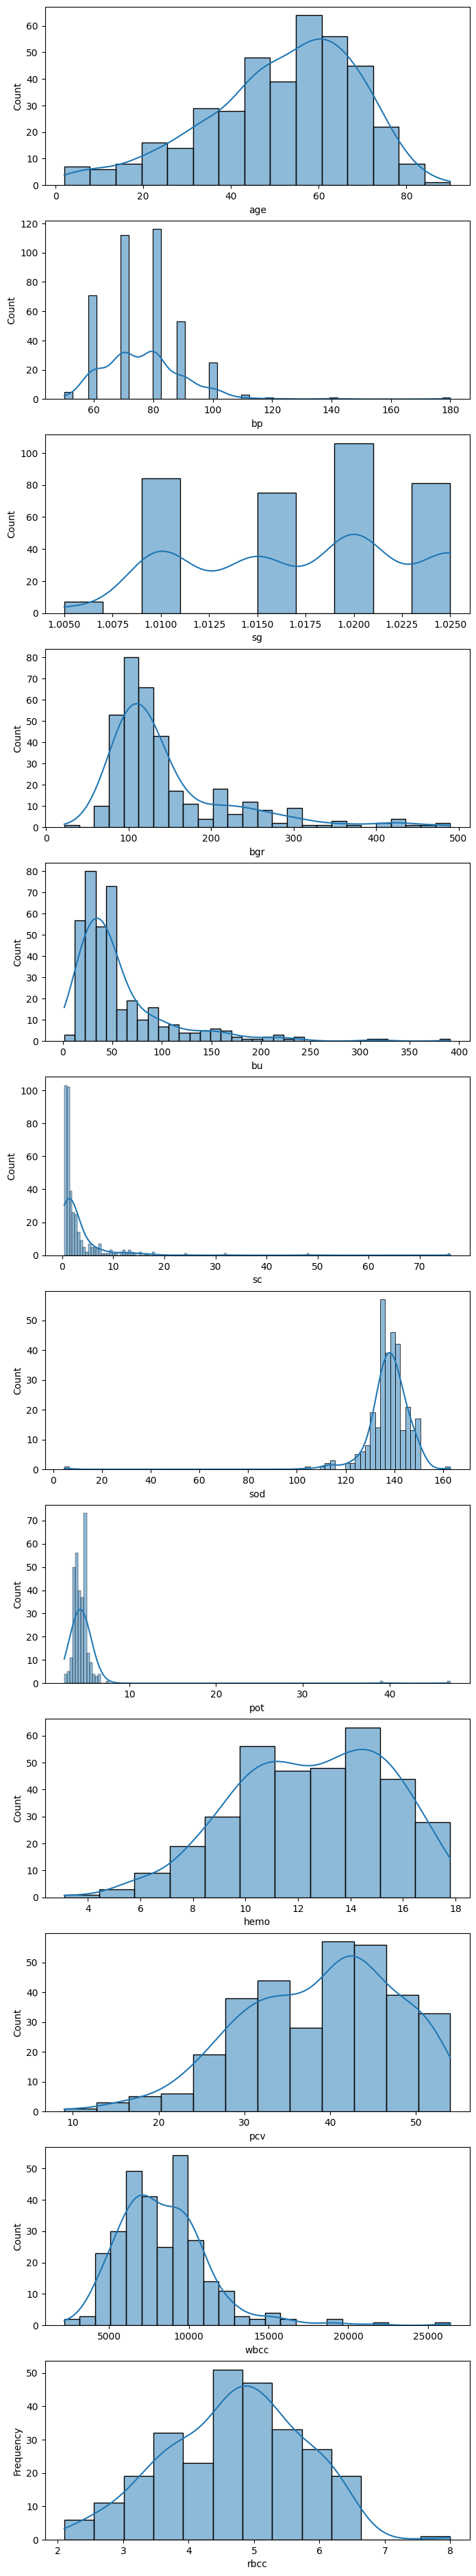
\includegraphics{Assignment6_Final version_files/figure-pdf/cell-14-output-1.png}

\begin{Shaded}
\begin{Highlighting}[]

\ControlFlowTok{for}\NormalTok{ i }\KeywordTok{in} \BuiltInTok{range}\NormalTok{(}\BuiltInTok{len}\NormalTok{(categorcal\_cols)):}
\NormalTok{    plt.figure(figsize}\OperatorTok{=}\NormalTok{(}\DecValTok{10}\NormalTok{, }\DecValTok{6}\NormalTok{))}
\NormalTok{    sns.countplot(x}\OperatorTok{=}\NormalTok{categorcal\_cols[i], data}\OperatorTok{=}\NormalTok{X)}
\NormalTok{    plt.title(}\StringTok{\textquotesingle{}Distribution of \textquotesingle{}}\OperatorTok{+}\NormalTok{ categorcal\_cols[i])}
\NormalTok{    plt.xlabel(}\StringTok{\textquotesingle{}Categories\textquotesingle{}}\NormalTok{)}
\NormalTok{    plt.ylabel(}\StringTok{\textquotesingle{}Count\textquotesingle{}}\NormalTok{)}
\NormalTok{    plt.xticks(rotation}\OperatorTok{=}\DecValTok{45}\NormalTok{)  }\CommentTok{\# Rotate x{-}axis labels for better readability if needed}
\NormalTok{    plt.show()}
\end{Highlighting}
\end{Shaded}

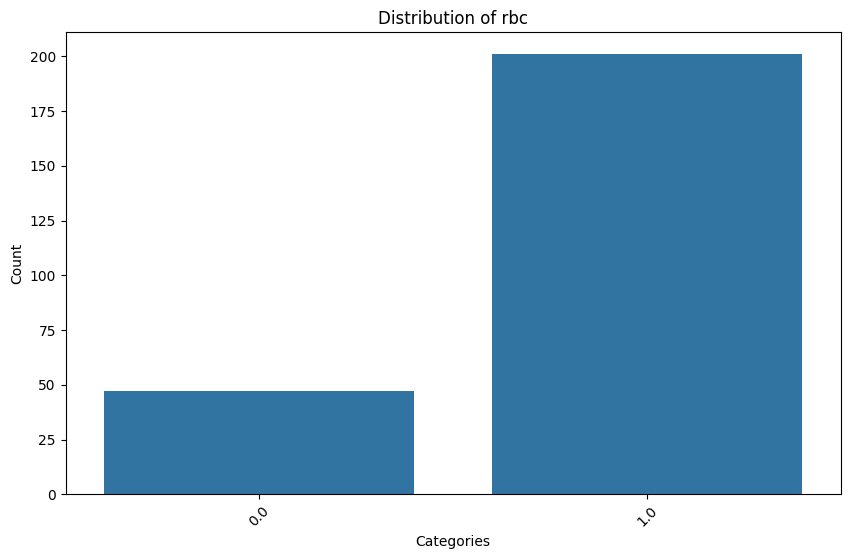
\includegraphics{Assignment6_Final version_files/figure-pdf/cell-15-output-1.png}

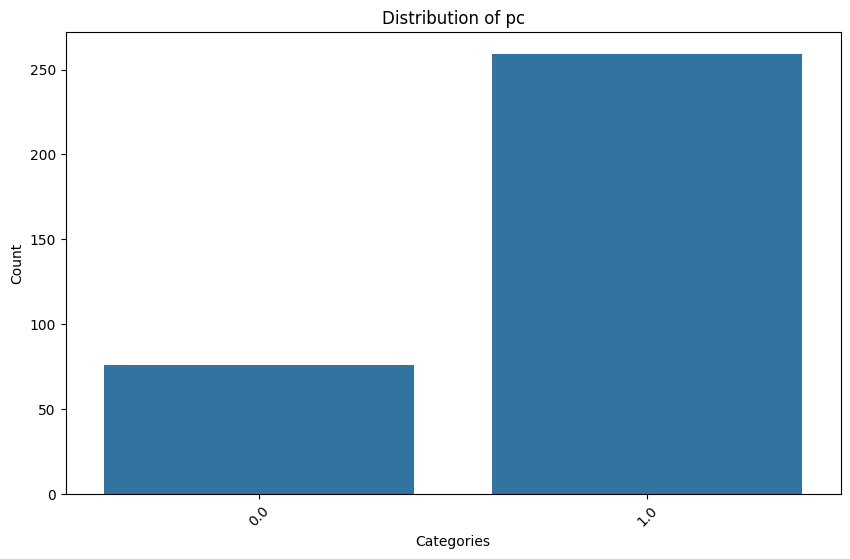
\includegraphics{Assignment6_Final version_files/figure-pdf/cell-15-output-2.png}

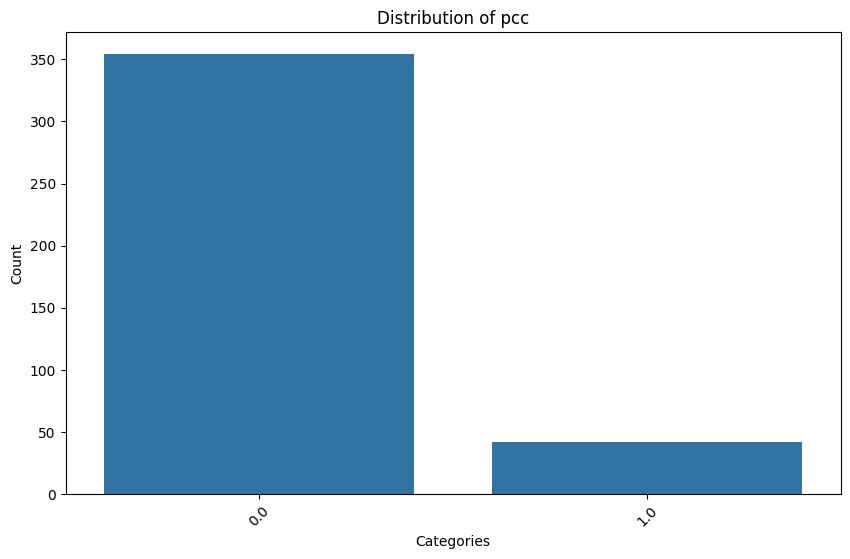
\includegraphics{Assignment6_Final version_files/figure-pdf/cell-15-output-3.png}

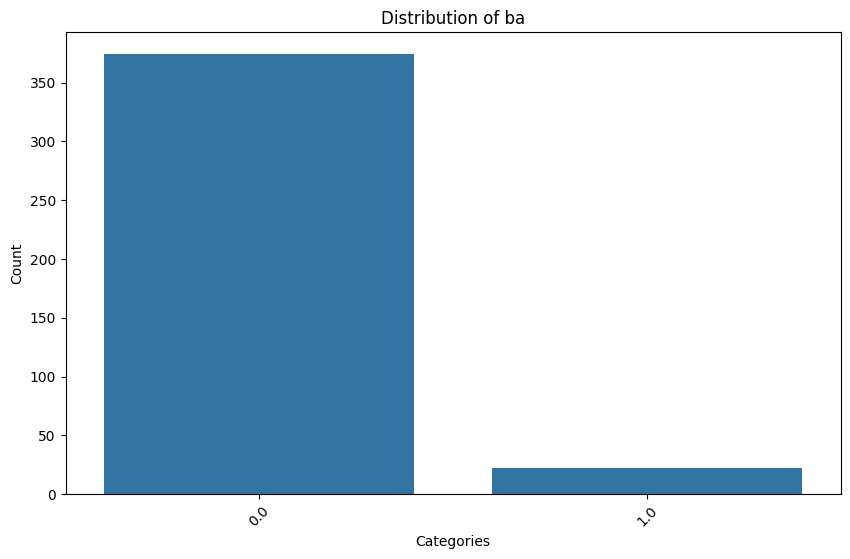
\includegraphics{Assignment6_Final version_files/figure-pdf/cell-15-output-4.png}

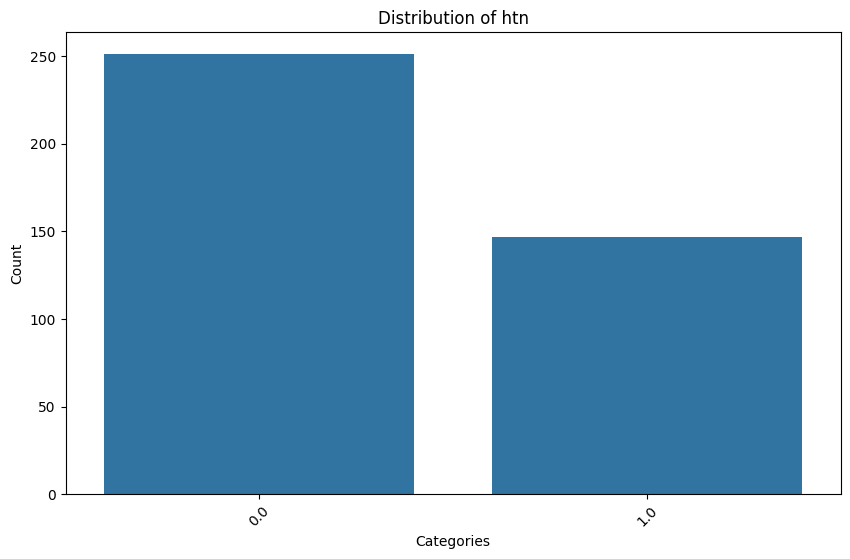
\includegraphics{Assignment6_Final version_files/figure-pdf/cell-15-output-5.png}

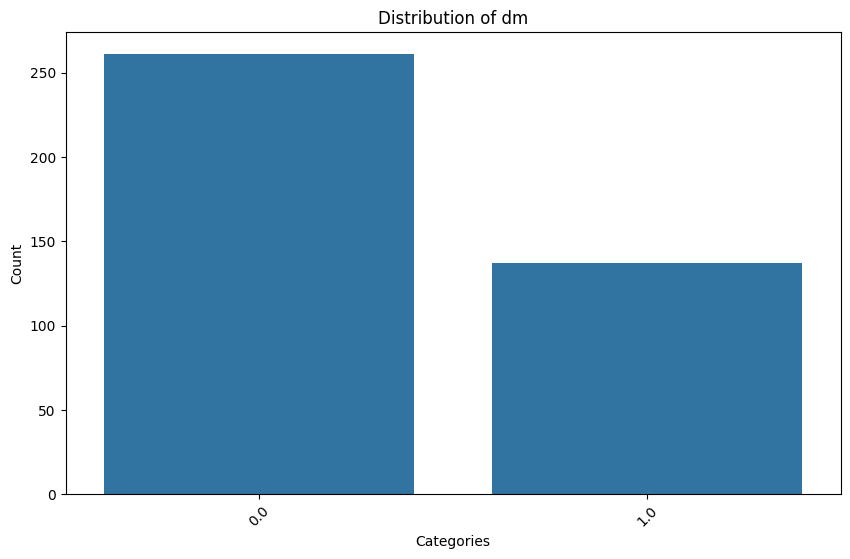
\includegraphics{Assignment6_Final version_files/figure-pdf/cell-15-output-6.png}

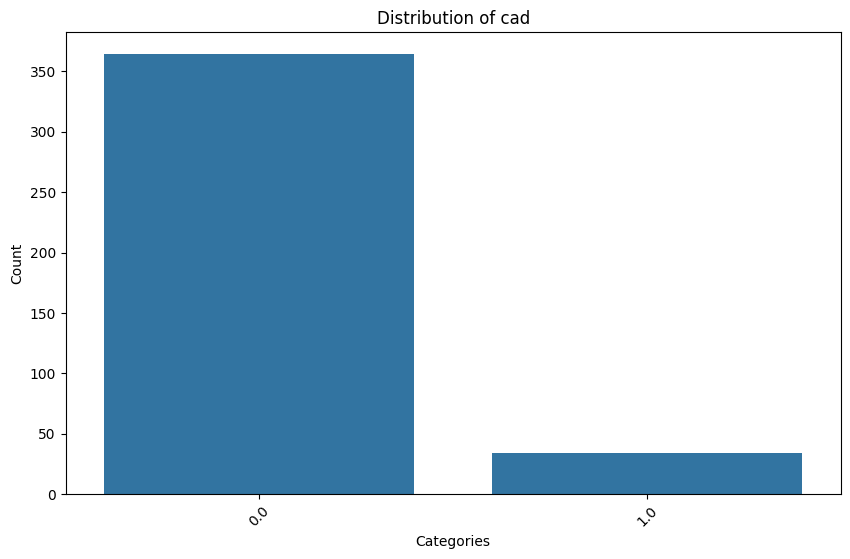
\includegraphics{Assignment6_Final version_files/figure-pdf/cell-15-output-7.png}

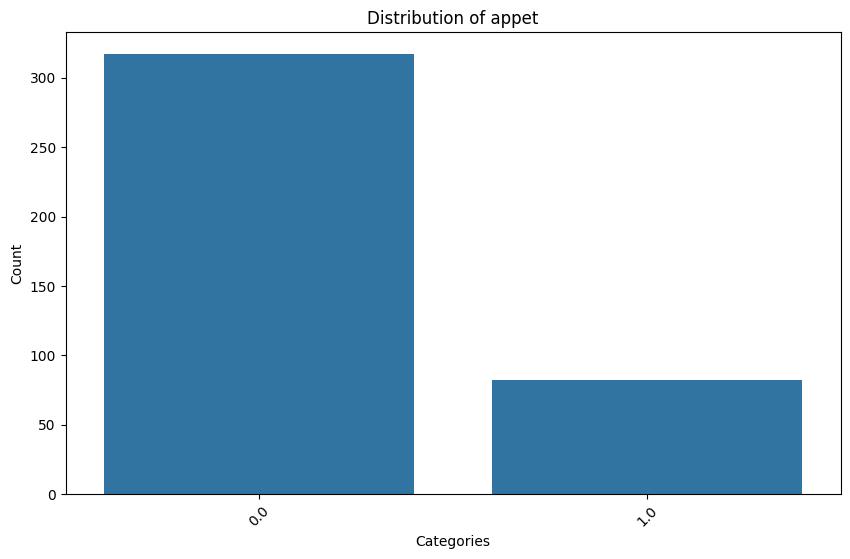
\includegraphics{Assignment6_Final version_files/figure-pdf/cell-15-output-8.png}

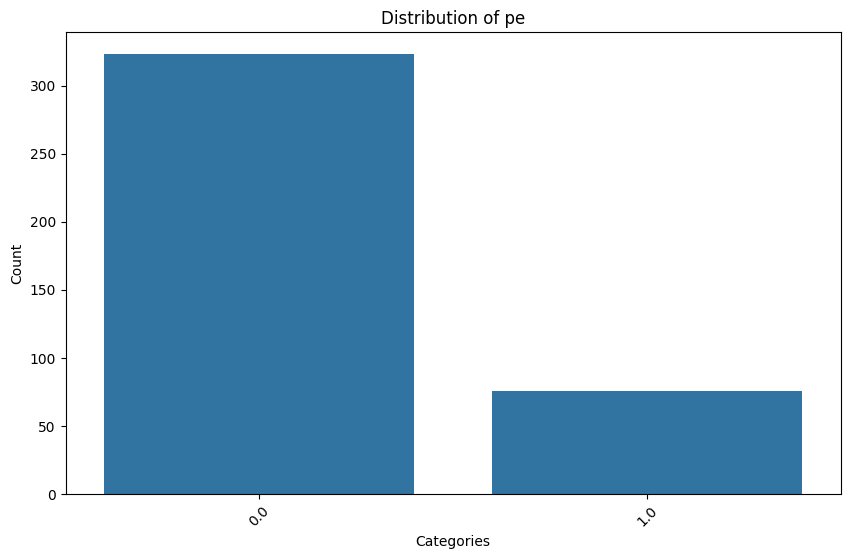
\includegraphics{Assignment6_Final version_files/figure-pdf/cell-15-output-9.png}

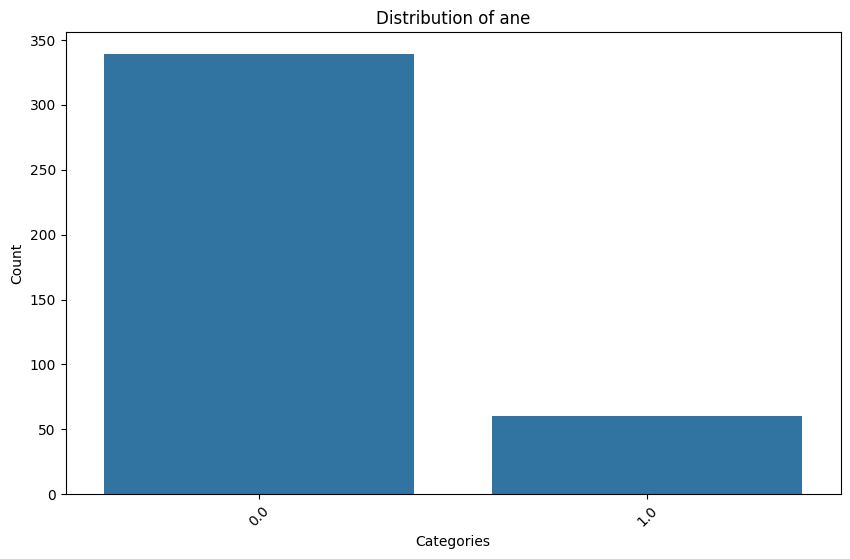
\includegraphics{Assignment6_Final version_files/figure-pdf/cell-15-output-10.png}

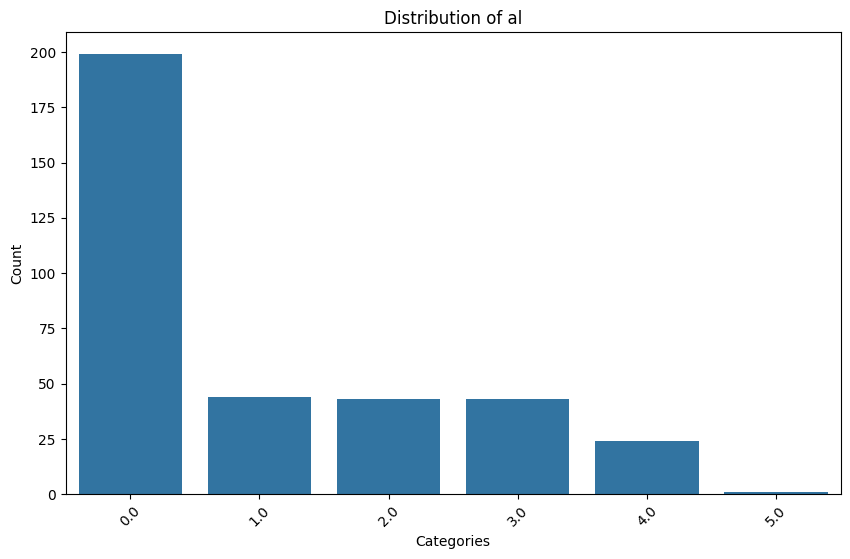
\includegraphics{Assignment6_Final version_files/figure-pdf/cell-15-output-11.png}

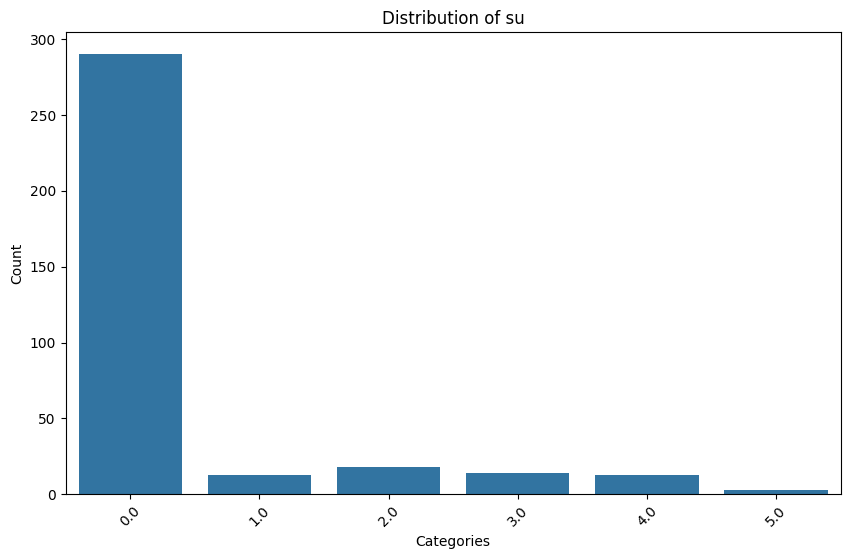
\includegraphics{Assignment6_Final version_files/figure-pdf/cell-15-output-12.png}

We standardlize numerical columns here, and we will not use them untill
we train our SVM model.

\begin{Shaded}
\begin{Highlighting}[]

\ImportTok{from}\NormalTok{ sklearn.preprocessing }\ImportTok{import}\NormalTok{ StandardScaler}
\NormalTok{scaler }\OperatorTok{=}\NormalTok{ StandardScaler()}
\NormalTok{StandardCol}\OperatorTok{=}\NormalTok{X}
\NormalTok{StandardCol[numerical\_cols] }\OperatorTok{=}\NormalTok{ scaler.fit\_transform(StandardCol[numerical\_cols])}
\NormalTok{StandardCol[numerical\_cols].describe().T}
\end{Highlighting}
\end{Shaded}

\begin{longtable}[]{@{}lllllllll@{}}
\toprule\noalign{}
& count & mean & std & min & 25\% & 50\% & 75\% & max \\
\midrule\noalign{}
\endhead
\bottomrule\noalign{}
\endlastfoot
age & 391.0 & 9.994847e-17 & 1.001281 & -2.885708 & -0.553039 & 0.205078
& 0.759087 & 2.246163 \\
bp & 388.0 & -2.380684e-16 & 1.001291 & -1.936857 & -0.473370 & 0.258373
& 0.258373 & 7.575807 \\
sg & 353.0 & 2.415443e-15 & 1.001419 & -2.173584 & -1.297699 & 0.454071
& 0.454071 & 1.329955 \\
bgr & 356.0 & -1.796316e-16 & 1.001407 & -1.591967 & -0.619380 &
-0.341498 & 0.189004 & 4.319341 \\
bu & 381.0 & -3.729883e-17 & 1.001315 & -1.108830 & -0.603246 &
-0.305843 & 0.170001 & 6.613723 \\
sc & 383.0 & 0.000000e+00 & 1.001308 & -0.466102 & -0.378897 & -0.309133
& -0.047519 & 12.719271 \\
sod & 313.0 & 2.270105e-17 & 1.001601 & -12.800936 & -0.243334 &
0.045347 & 0.430254 & 2.451017 \\
pot & 312.0 & -7.970832e-17 & 1.001606 & -0.667102 & -0.259423 &
-0.071263 & 0.085536 & 13.288071 \\
hemo & 348.0 & 4.083579e-17 & 1.001440 & -3.241109 & -0.765520 &
0.042485 & 0.850490 & 1.813219 \\
pcv & 329.0 & 1.295823e-16 & 1.001523 & -3.329218 & -0.766953 & 0.124270
& 0.681284 & 1.683910 \\
wbcc & 294.0 & 1.450087e-16 & 1.001705 & -2.111312 & -0.648460 &
-0.138162 & 0.474195 & 6.121486 \\
rbcc & 269.0 & 8.452553e-16 & 1.001864 & -2.547777 & -0.788961 &
0.090447 & 0.676719 & 3.217231 \\
\end{longtable}

There are a total of 400 records. The age of these records are mostly
distributed among 40 to 80. For variable ``sc'',``bu'',``bgr'' and
``wbcc'', they are left-skewed. For variable ``pcv'', and ``hemo'', they
are right-skewed.

\section{4}\label{section-2}

The heatmap below shows the corrlations of the combinations of the
variables.

\begin{Shaded}
\begin{Highlighting}[]
\CommentTok{\# Plot heatmap of covariance matrix}
\NormalTok{plt.figure(figsize}\OperatorTok{=}\NormalTok{(}\DecValTok{10}\NormalTok{, }\DecValTok{8}\NormalTok{))}
\NormalTok{sns.heatmap(X[numerical\_cols].corr(),annot}\OperatorTok{=}\VariableTok{True}\NormalTok{)}
\NormalTok{plt.title(}\StringTok{\textquotesingle{}Covariance Matrix Heatmap\textquotesingle{}}\NormalTok{)}
\NormalTok{plt.show()}
\end{Highlighting}
\end{Shaded}

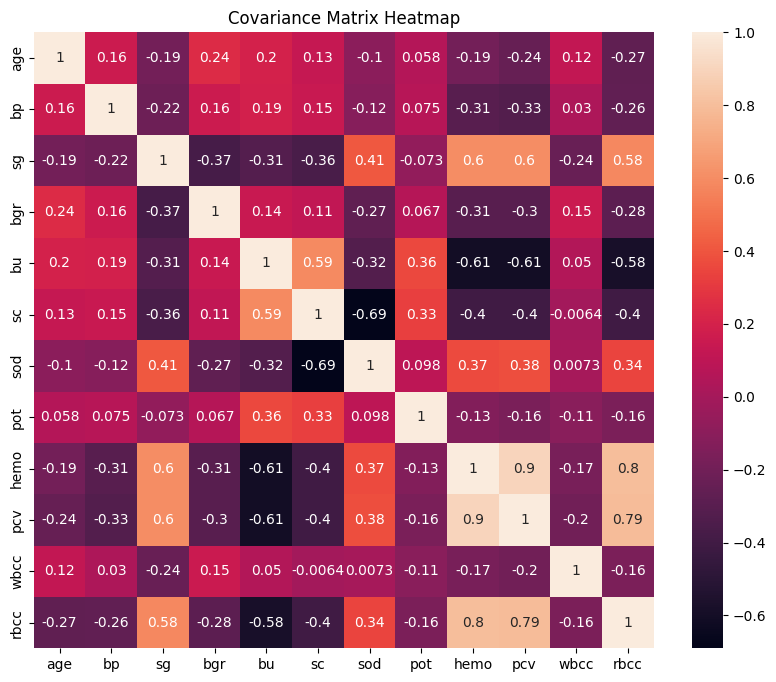
\includegraphics{Assignment6_Final version_files/figure-pdf/cell-17-output-1.png}

Relation between ``sod'' and ``sc'' has the most negative corrleation;

Relation between ``hemo'' and ``rbcc'' has the most positive
corrleation.;

Relation between ``wbcc'' and ``bp'' has the smallest corrleation, which
means they are close to a independent relation.

\section{5}\label{section-3}

For quantitative variables, we replace the missing values by the mean of
each column. For categorical variables, we replace the missing values by
the most frequently appeared value in each column. However, we will not
process the missing values now since Decision Tree can accept missing
values. We will impute missing values before we use SVM.

The related code is at page 41.

\section{6 Outlier Analysis}\label{outlier-analysis}

From the histogrms below we obtain that some outliers do exist. However,
we decide not to remove them because a certain value in a certain column
may be influenced by other variables, we cannot find a clear method or
rule to remove the outliers though we got a heatmap. Also, some of the
medical data may be conclusive in determing the disease, so we think
keep these outlier here is not necessary.

\begin{Shaded}
\begin{Highlighting}[]

\ControlFlowTok{for}\NormalTok{ col }\KeywordTok{in}\NormalTok{ numerical\_cols:}
\NormalTok{    plt.figure(figsize}\OperatorTok{=}\NormalTok{(}\DecValTok{6}\NormalTok{, }\DecValTok{4}\NormalTok{))}
\NormalTok{    sns.boxplot(x}\OperatorTok{=}\NormalTok{X[col])}
\NormalTok{    plt.title(}\SpecialStringTok{f\textquotesingle{}Box Plot of }\SpecialCharTok{\{}\NormalTok{col}\SpecialCharTok{\}}\SpecialStringTok{\textquotesingle{}}\NormalTok{)}
\NormalTok{    plt.xlabel(col)}
\NormalTok{    plt.show()}
\end{Highlighting}
\end{Shaded}

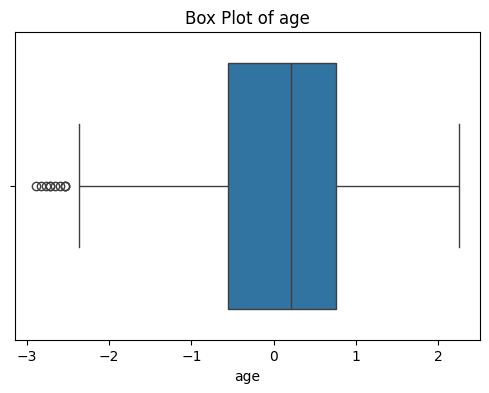
\includegraphics{Assignment6_Final version_files/figure-pdf/cell-18-output-1.png}

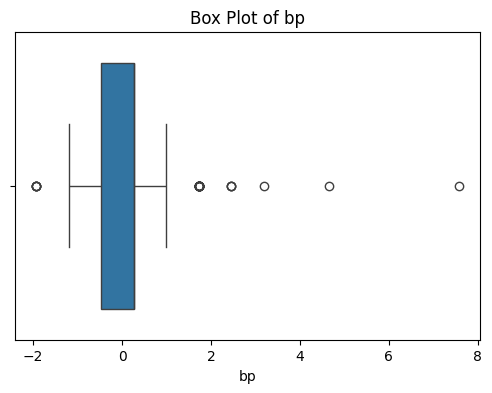
\includegraphics{Assignment6_Final version_files/figure-pdf/cell-18-output-2.png}

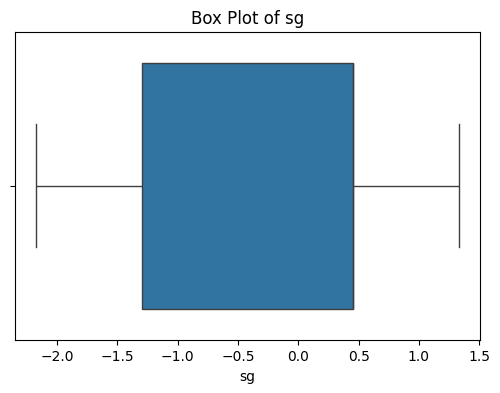
\includegraphics{Assignment6_Final version_files/figure-pdf/cell-18-output-3.png}

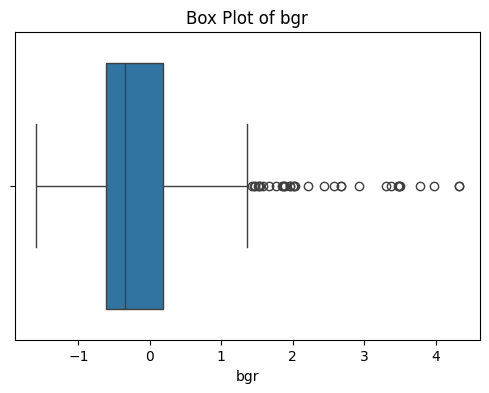
\includegraphics{Assignment6_Final version_files/figure-pdf/cell-18-output-4.png}

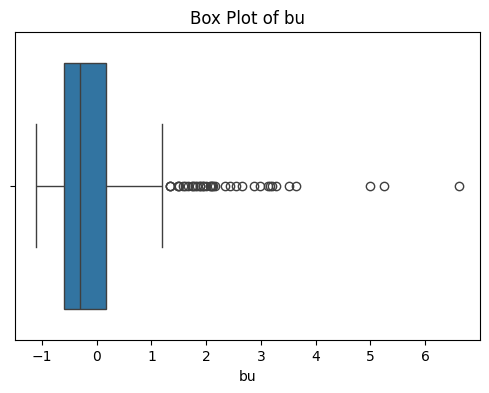
\includegraphics{Assignment6_Final version_files/figure-pdf/cell-18-output-5.png}

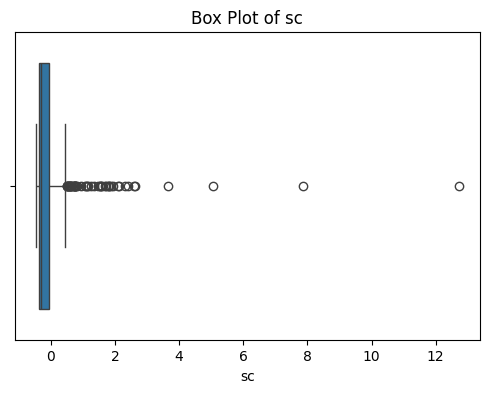
\includegraphics{Assignment6_Final version_files/figure-pdf/cell-18-output-6.png}

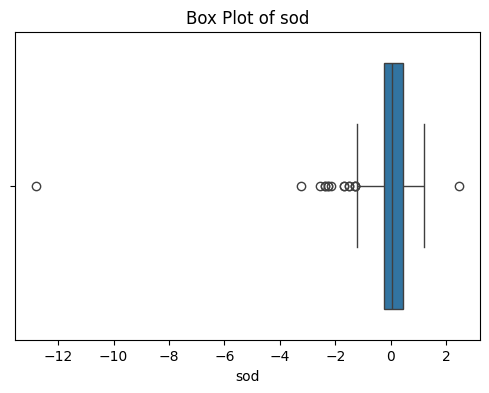
\includegraphics{Assignment6_Final version_files/figure-pdf/cell-18-output-7.png}

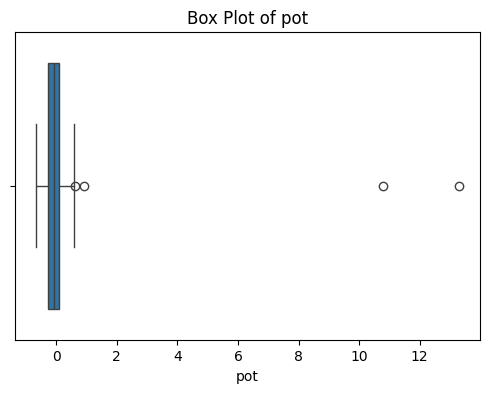
\includegraphics{Assignment6_Final version_files/figure-pdf/cell-18-output-8.png}

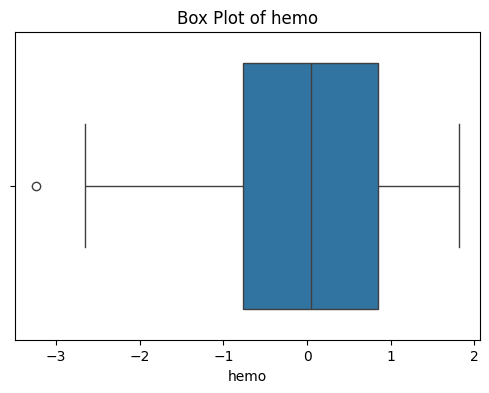
\includegraphics{Assignment6_Final version_files/figure-pdf/cell-18-output-9.png}

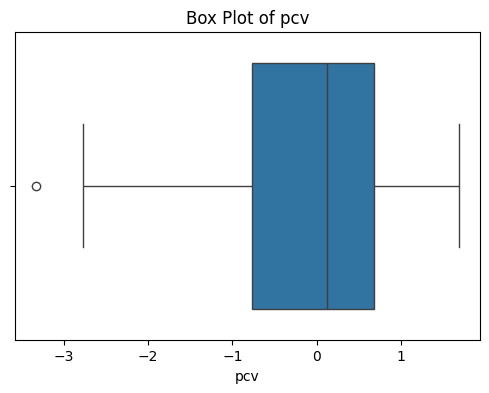
\includegraphics{Assignment6_Final version_files/figure-pdf/cell-18-output-10.png}

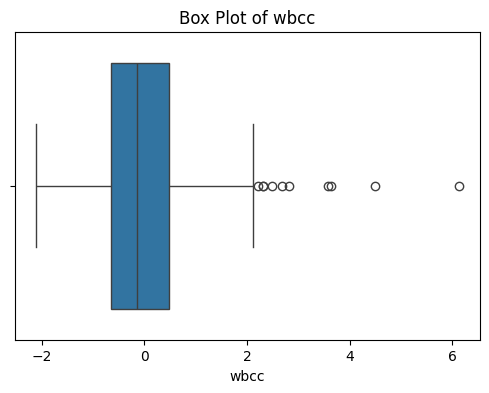
\includegraphics{Assignment6_Final version_files/figure-pdf/cell-18-output-11.png}

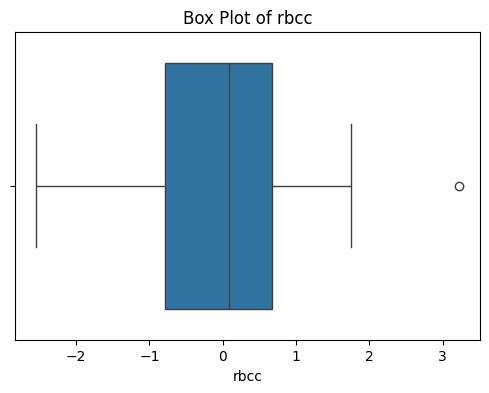
\includegraphics{Assignment6_Final version_files/figure-pdf/cell-18-output-12.png}

\section{7. Subgrouping}\label{subgrouping}

\begin{Shaded}
\begin{Highlighting}[]
\NormalTok{combined\_df }\OperatorTok{=}\NormalTok{ pd.concat([X, y], axis}\OperatorTok{=}\DecValTok{1}\NormalTok{)}

\CommentTok{\# Drop rows with missing values}
\NormalTok{combined\_df }\OperatorTok{=}\NormalTok{ combined\_df.dropna()}

\NormalTok{new\_y}\OperatorTok{=}\NormalTok{combined\_df[}\StringTok{"class"}\NormalTok{]}
\NormalTok{new\_X }\OperatorTok{=}\NormalTok{ combined\_df.drop(columns}\OperatorTok{=}\NormalTok{[}\StringTok{"class"}\NormalTok{])}
\end{Highlighting}
\end{Shaded}

\begin{Shaded}
\begin{Highlighting}[]
\BuiltInTok{print}\NormalTok{(new\_y.shape)}
\BuiltInTok{print}\NormalTok{(new\_X.shape)}
\end{Highlighting}
\end{Shaded}

\begin{verbatim}
(158,)
(158, 24)
\end{verbatim}

\begin{Shaded}
\begin{Highlighting}[]
\NormalTok{range\_n\_clusters }\OperatorTok{=}\NormalTok{ [}\DecValTok{2}\NormalTok{, }\DecValTok{3}\NormalTok{, }\DecValTok{4}\NormalTok{, }\DecValTok{5}\NormalTok{, }\DecValTok{6}\NormalTok{]}
\ControlFlowTok{for}\NormalTok{ n\_clusters }\KeywordTok{in}\NormalTok{ range\_n\_clusters:}
\NormalTok{    km }\OperatorTok{=}\NormalTok{ KMeans(n\_clusters}\OperatorTok{=}\NormalTok{n\_clusters, n\_init}\OperatorTok{=}\DecValTok{20}\NormalTok{, random\_state}\OperatorTok{=}\DecValTok{0}\NormalTok{)}
\NormalTok{    labels }\OperatorTok{=}\NormalTok{ km.fit\_predict(new\_X)}
    
\NormalTok{    silhouette\_avg }\OperatorTok{=}\NormalTok{ silhouette\_score(new\_X, labels)}
\NormalTok{    sample\_silhouette\_values }\OperatorTok{=}\NormalTok{ silhouette\_samples(new\_X, labels)}
\NormalTok{    fig, ax1 }\OperatorTok{=}\NormalTok{ plt.subplots(}\DecValTok{1}\NormalTok{, }\DecValTok{1}\NormalTok{)}
\NormalTok{    fig.set\_size\_inches(}\DecValTok{18}\NormalTok{, }\DecValTok{7}\NormalTok{)}
\NormalTok{    ax1.set\_xlim([}\OperatorTok{{-}}\FloatTok{0.3}\NormalTok{, }\DecValTok{1}\NormalTok{])}

\NormalTok{    y\_lower }\OperatorTok{=} \DecValTok{10}
    
    \ControlFlowTok{for}\NormalTok{ i }\KeywordTok{in} \BuiltInTok{range}\NormalTok{(n\_clusters):}
\NormalTok{        ith\_cluster\_silhouette\_values }\OperatorTok{=}\NormalTok{ sample\_silhouette\_values[labels }\OperatorTok{==}\NormalTok{ i]}
\NormalTok{        ith\_cluster\_silhouette\_values.sort()}

\NormalTok{        size\_cluster\_i }\OperatorTok{=}\NormalTok{ ith\_cluster\_silhouette\_values.shape[}\DecValTok{0}\NormalTok{]}
\NormalTok{        y\_upper }\OperatorTok{=}\NormalTok{ y\_lower }\OperatorTok{+}\NormalTok{ size\_cluster\_i}

        \CommentTok{\# Use the colormap for coloring}
\NormalTok{        color }\OperatorTok{=}\NormalTok{ cm.nipy\_spectral(}\BuiltInTok{float}\NormalTok{(i) }\OperatorTok{/}\NormalTok{ n\_clusters)}
\NormalTok{        ax1.fill\_betweenx(}
\NormalTok{            y}\OperatorTok{=}\NormalTok{np.arange(y\_lower, y\_upper),}
\NormalTok{            x1}\OperatorTok{=}\DecValTok{0}\NormalTok{,}
\NormalTok{            x2}\OperatorTok{=}\NormalTok{ith\_cluster\_silhouette\_values,}
\NormalTok{            facecolor}\OperatorTok{=}\NormalTok{color,}
\NormalTok{            edgecolor}\OperatorTok{=}\NormalTok{color,}
\NormalTok{            alpha}\OperatorTok{=}\FloatTok{0.7}\NormalTok{,}
\NormalTok{        )}

\NormalTok{        ax1.text(}\OperatorTok{{-}}\FloatTok{0.05}\NormalTok{, y\_lower }\OperatorTok{+} \FloatTok{0.5} \OperatorTok{*}\NormalTok{ size\_cluster\_i, }\BuiltInTok{str}\NormalTok{(i))}

\NormalTok{        y\_lower }\OperatorTok{=}\NormalTok{ y\_upper }\OperatorTok{+} \DecValTok{10}  

\NormalTok{    ax1.set\_title(}\StringTok{"The silhouette plot for various clusters"}\NormalTok{)}
\NormalTok{    ax1.set\_xlabel(}\StringTok{"The silhouette coefficient values"}\NormalTok{)}
\NormalTok{    ax1.set\_ylabel(}\StringTok{"Cluster label"}\NormalTok{)}

\NormalTok{    ax1.axvline(x}\OperatorTok{=}\NormalTok{silhouette\_avg, color}\OperatorTok{=}\StringTok{"red"}\NormalTok{, linestyle}\OperatorTok{=}\StringTok{"{-}{-}"}\NormalTok{)}
\NormalTok{    plt.title(}
        \StringTok{"Silhouette analysis for KMeans clustering on sample data with n\_clusters = }\SpecialCharTok{\%d}\StringTok{"}
        \OperatorTok{\%}\NormalTok{ n\_clusters,}
\NormalTok{        fontsize}\OperatorTok{=}\DecValTok{14}\NormalTok{,}
\NormalTok{        fontweight}\OperatorTok{=}\StringTok{"bold"}\NormalTok{,}
\NormalTok{    )}

\NormalTok{plt.show()}
\end{Highlighting}
\end{Shaded}

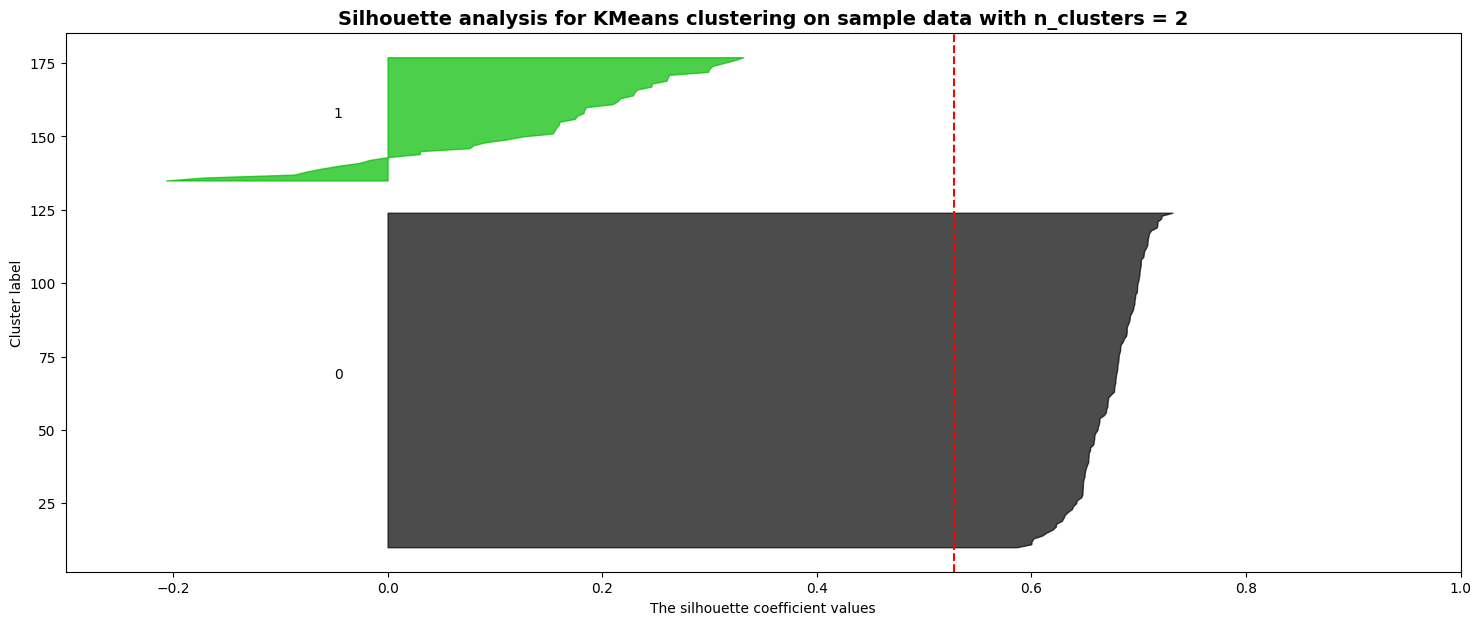
\includegraphics{Assignment6_Final version_files/figure-pdf/cell-21-output-1.png}

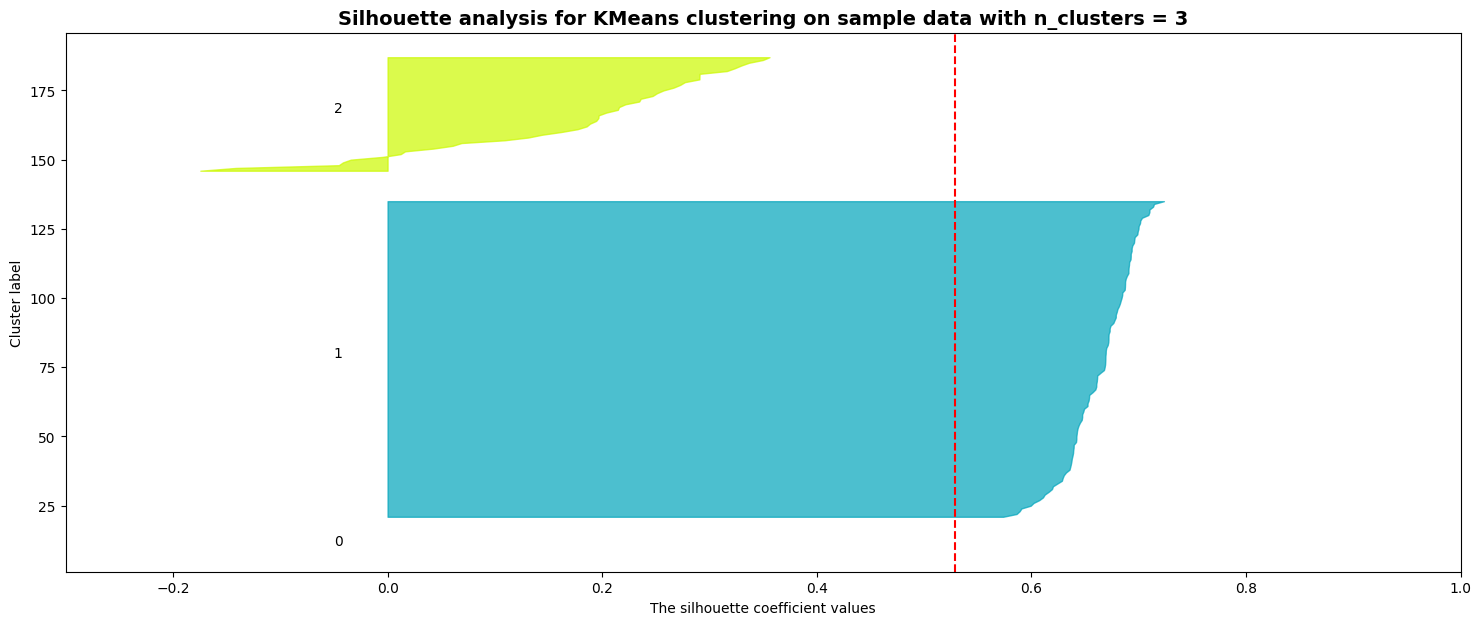
\includegraphics{Assignment6_Final version_files/figure-pdf/cell-21-output-2.png}

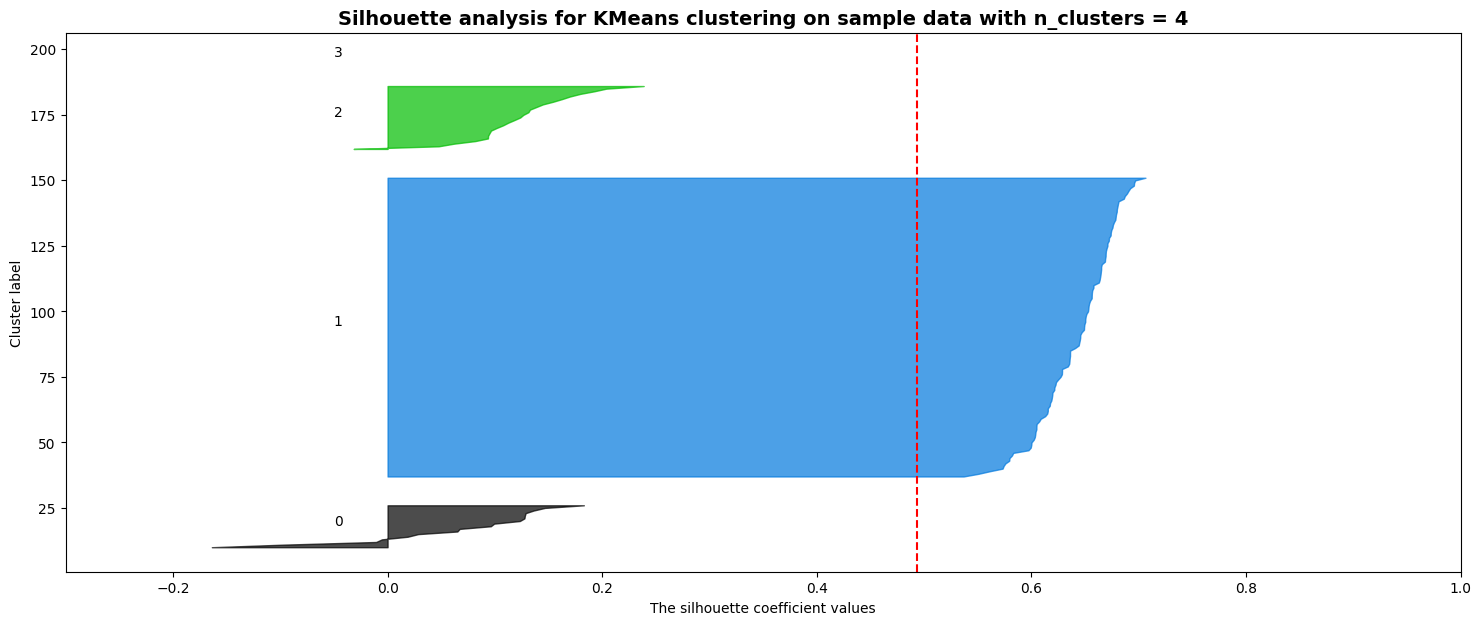
\includegraphics{Assignment6_Final version_files/figure-pdf/cell-21-output-3.png}

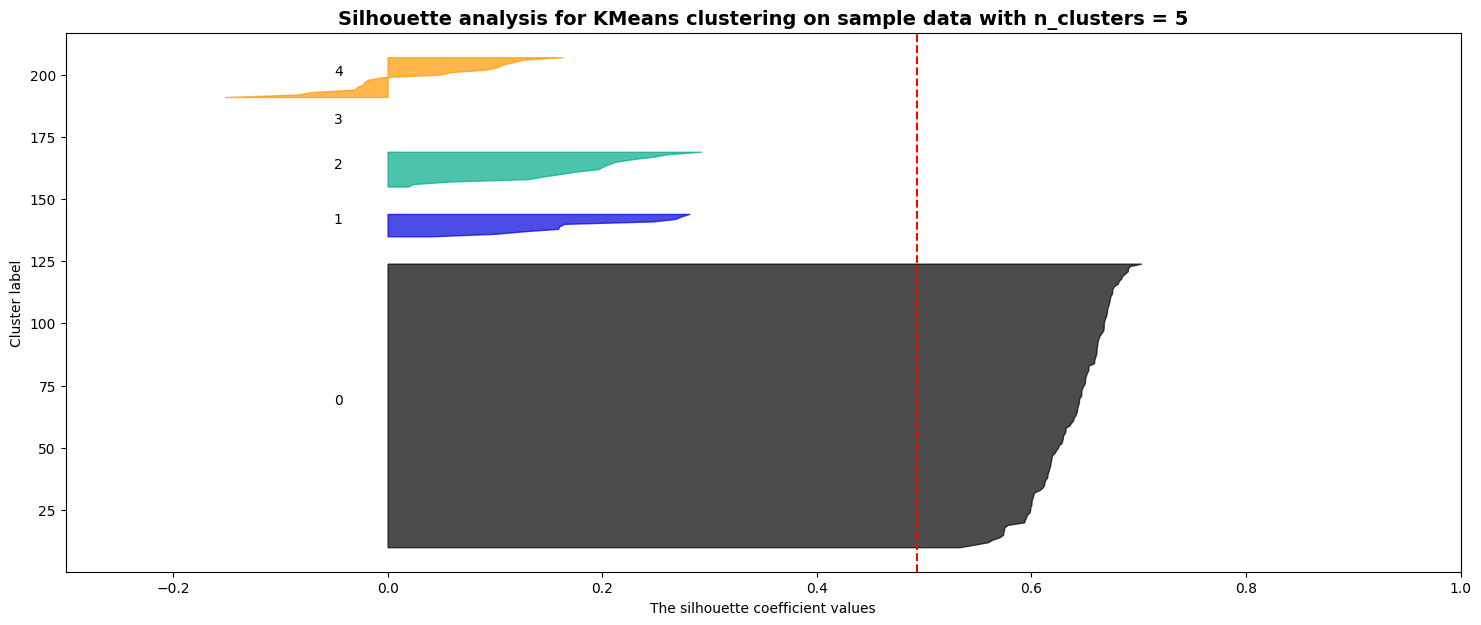
\includegraphics{Assignment6_Final version_files/figure-pdf/cell-21-output-4.png}

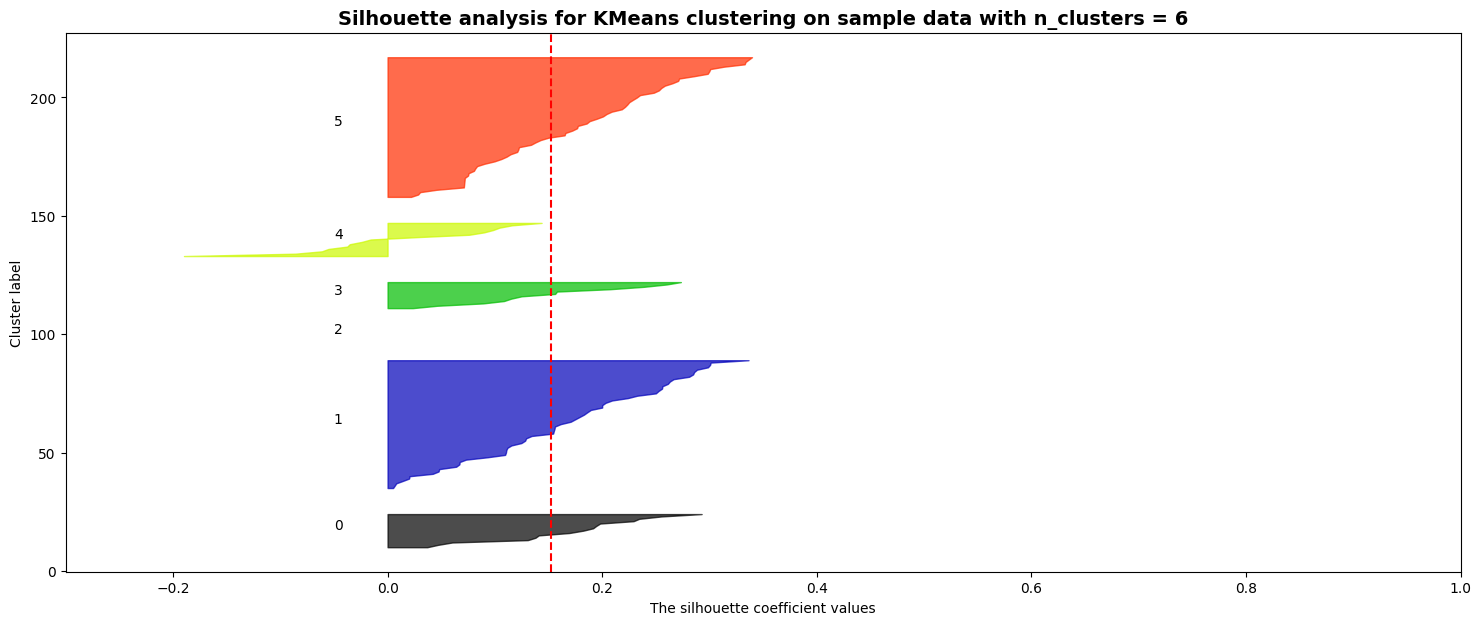
\includegraphics{Assignment6_Final version_files/figure-pdf/cell-21-output-5.png}

\begin{Shaded}
\begin{Highlighting}[]
\NormalTok{k\_values }\OperatorTok{=} \BuiltInTok{range}\NormalTok{(}\DecValTok{2}\NormalTok{, }\DecValTok{8}\NormalTok{) }\CommentTok{\# You can adjust this range as needed}
\CommentTok{\# Initialize lists to store silhouette scores}
\NormalTok{silhouette\_scores }\OperatorTok{=}\NormalTok{ []}
\CommentTok{\# Iterate through different values of k}
\ControlFlowTok{for}\NormalTok{ k }\KeywordTok{in}\NormalTok{ k\_values:}
\CommentTok{\# Fit KMeans clustering to the data}
\NormalTok{    kmeans }\OperatorTok{=}\NormalTok{ KMeans(n\_clusters}\OperatorTok{=}\NormalTok{k, n\_init }\OperatorTok{=} \DecValTok{20}\NormalTok{,random\_state}\OperatorTok{=}\DecValTok{0}\NormalTok{)}
\NormalTok{    kmeans.fit(new\_X)}
\CommentTok{\# Compute the silhouette score}
\NormalTok{    silhouette\_avg }\OperatorTok{=}\NormalTok{ silhouette\_score(new\_X, kmeans.labels\_)}
\NormalTok{    silhouette\_scores.append(silhouette\_avg)}
\CommentTok{\# Plot silhouette scores against k}
\NormalTok{plt.plot(k\_values, silhouette\_scores, marker}\OperatorTok{=}\StringTok{\textquotesingle{}o\textquotesingle{}}\NormalTok{)}
\NormalTok{plt.xlabel(}\StringTok{\textquotesingle{}Number of Clusters\textquotesingle{}}\NormalTok{)}
\NormalTok{plt.ylabel(}\StringTok{\textquotesingle{}Silhouette Score\textquotesingle{}}\NormalTok{)}
\NormalTok{plt.title(}\StringTok{\textquotesingle{}Silhouette Scores\textquotesingle{}}\NormalTok{)}
\NormalTok{plt.show()}
\end{Highlighting}
\end{Shaded}

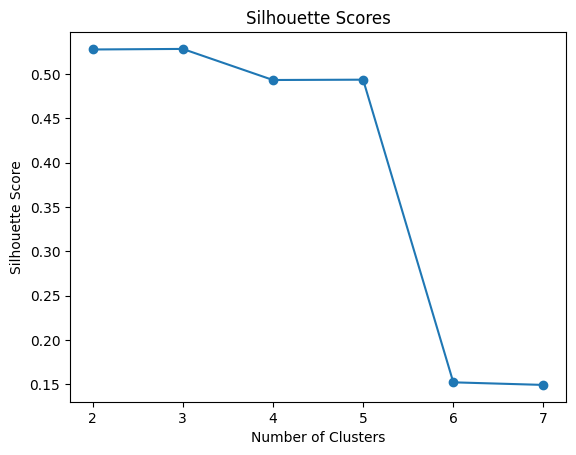
\includegraphics{Assignment6_Final version_files/figure-pdf/cell-22-output-1.png}

We observe that when k=2, it has the best silhouette score. This result
also aligns with the common sense the dataset.

\begin{Shaded}
\begin{Highlighting}[]
\NormalTok{combined\_df }\OperatorTok{=}\NormalTok{ pd.concat([X, y], axis}\OperatorTok{=}\DecValTok{1}\NormalTok{)}

\CommentTok{\# Drop rows with missing values}
\NormalTok{combined\_df }\OperatorTok{=}\NormalTok{ combined\_df.dropna()}


\NormalTok{combined\_df[}\StringTok{"class"}\NormalTok{]}

\end{Highlighting}
\end{Shaded}

\begin{verbatim}
3         ckd
9         ckd
11        ckd
14        ckd
20        ckd
        ...  
395    notckd
396    notckd
397    notckd
398    notckd
399    notckd
Name: class, Length: 158, dtype: object
\end{verbatim}

\section{8. Data Splitting}\label{data-splitting}

\begin{Shaded}
\begin{Highlighting}[]
\NormalTok{X\_train, X\_test, y\_train, y\_test }\OperatorTok{=}\NormalTok{ train\_test\_split(}
\NormalTok{    X, y, test\_size}\OperatorTok{=}\FloatTok{0.3}\NormalTok{, random\_state}\OperatorTok{=}\DecValTok{1}\NormalTok{, stratify}\OperatorTok{=}\NormalTok{y)}
\end{Highlighting}
\end{Shaded}

\section{9.}\label{section-4}

Like we mentioned before, we will be using Decision Tree and SVM for
classification. We choose these two methods after we explore the whole
dataset.

\begin{Shaded}
\begin{Highlighting}[]
\NormalTok{cs\_dt }\OperatorTok{=}\NormalTok{ DecisionTreeClassifier(}
\NormalTok{    max\_depth }\OperatorTok{=}\DecValTok{30}\NormalTok{, }
\NormalTok{    random\_state}\OperatorTok{=}\DecValTok{1}
\NormalTok{) }
\end{Highlighting}
\end{Shaded}

\begin{Shaded}
\begin{Highlighting}[]
\NormalTok{cs\_dt.fit(X\_train, y\_train)}

\NormalTok{plot\_tree(}
\NormalTok{    cs\_dt, }
\NormalTok{    max\_depth}\OperatorTok{=} \DecValTok{30}\NormalTok{, }
\NormalTok{    feature\_names }\OperatorTok{=}\NormalTok{ X\_train.columns.tolist(), }
\NormalTok{    class\_names}\OperatorTok{=}\NormalTok{[}\StringTok{\textquotesingle{}notckd\textquotesingle{}}\NormalTok{, }\StringTok{\textquotesingle{}ckd\textquotesingle{}}\NormalTok{],}
\NormalTok{    filled}\OperatorTok{=}\VariableTok{True}
\NormalTok{)}

\NormalTok{pred\_DT }\OperatorTok{=}\NormalTok{ cs\_dt.predict(X\_test)}
\NormalTok{pred\_DT[:}\DecValTok{5}\NormalTok{]}

\end{Highlighting}
\end{Shaded}

\begin{verbatim}
array(['ckd', 'ckd', 'ckd', 'notckd', 'notckd'], dtype=object)
\end{verbatim}

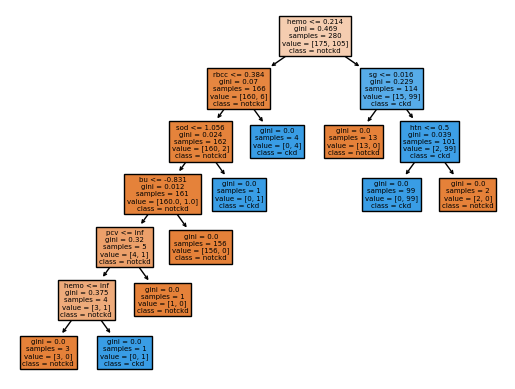
\includegraphics{Assignment6_Final version_files/figure-pdf/cell-26-output-2.png}

\section{10. Performance Metrics}\label{performance-metrics}

We use the confucsion matrix as well as classification\_report to
measure our accuracy.

\begin{Shaded}
\begin{Highlighting}[]

\NormalTok{cm\_DT }\OperatorTok{=}\NormalTok{ pd.DataFrame(confusion\_matrix(y\_test, pred\_DT), index}\OperatorTok{=}\NormalTok{[}\StringTok{\textquotesingle{}No\textquotesingle{}}\NormalTok{, }\StringTok{\textquotesingle{}Yes\textquotesingle{}}\NormalTok{], columns}\OperatorTok{=}\NormalTok{[}\StringTok{\textquotesingle{}No\textquotesingle{}}\NormalTok{, }\StringTok{\textquotesingle{}Yes\textquotesingle{}}\NormalTok{])}
\NormalTok{cm\_DT.index.name }\OperatorTok{=} \StringTok{\textquotesingle{}True\textquotesingle{}}
\NormalTok{cm\_DT.columns.name }\OperatorTok{=} \StringTok{\textquotesingle{}Predicted\textquotesingle{}}


\BuiltInTok{print}\NormalTok{(cm\_DT)}
\BuiltInTok{print}\NormalTok{(cs\_dt.score(X\_test, y\_test))}
\BuiltInTok{print}\NormalTok{(classification\_report(y\_test, pred\_DT))}
\end{Highlighting}
\end{Shaded}

\begin{verbatim}
Predicted  No  Yes
True              
No         73    2
Yes         3   42
0.9583333333333334
              precision    recall  f1-score   support

         ckd       0.96      0.97      0.97        75
      notckd       0.95      0.93      0.94        45

    accuracy                           0.96       120
   macro avg       0.96      0.95      0.96       120
weighted avg       0.96      0.96      0.96       120
\end{verbatim}

\section{11.}\label{section-5}

Here we use two methods to improve the performance on decision tree.
First method we prune the tree. Second Method, we fit our data with
criterion=`entropy', we did some research, and we agree on using entropy
instead of ``gini'' is more suitable for this dataset, and its
performance also proves that.

\begin{Shaded}
\begin{Highlighting}[]
\NormalTok{path }\OperatorTok{=}\NormalTok{ cs\_dt.cost\_complexity\_pruning\_path(}
\NormalTok{    X\_train, }
\NormalTok{    y\_train}
\NormalTok{)}
\NormalTok{ccp\_alphas, impurities }\OperatorTok{=}\NormalTok{ path.ccp\_alphas, path.impurities}
\end{Highlighting}
\end{Shaded}

\begin{Shaded}
\begin{Highlighting}[]
\NormalTok{clfs }\OperatorTok{=}\NormalTok{ [] }\CommentTok{\# save fitted trees with different alphas}
\ControlFlowTok{for}\NormalTok{ ccp\_alpha }\KeywordTok{in}\NormalTok{ ccp\_alphas:}
\NormalTok{    clf }\OperatorTok{=}\NormalTok{ DecisionTreeClassifier(}
\NormalTok{        random\_state}\OperatorTok{=}\DecValTok{0}\NormalTok{, }
\NormalTok{        ccp\_alpha}\OperatorTok{=}\NormalTok{ccp\_alpha}
\NormalTok{        )}
\NormalTok{    clf.fit(X\_train, y\_train)}
\NormalTok{    clfs.append(clf)}
\end{Highlighting}
\end{Shaded}

\begin{Shaded}
\begin{Highlighting}[]
\NormalTok{depth }\OperatorTok{=}\NormalTok{ [clf.tree\_.max\_depth }\ControlFlowTok{for}\NormalTok{ clf }\KeywordTok{in}\NormalTok{ clfs]}
\NormalTok{depth}
\end{Highlighting}
\end{Shaded}

\begin{verbatim}
[5, 5, 3, 2, 2, 1, 0]
\end{verbatim}

\begin{Shaded}
\begin{Highlighting}[]
\NormalTok{test\_score }\OperatorTok{=}\NormalTok{ [clf.score(X\_test, y\_test) }\ControlFlowTok{for}\NormalTok{ clf }\KeywordTok{in}\NormalTok{ clfs]}
\NormalTok{plt.plot(depth, test\_score)}
\NormalTok{plt.xlabel(}\StringTok{\textquotesingle{}Depth\textquotesingle{}}\NormalTok{)}
\NormalTok{plt.ylabel(}\StringTok{\textquotesingle{}Accuracy\textquotesingle{}}\NormalTok{)}
\NormalTok{plt.show()}
\end{Highlighting}
\end{Shaded}

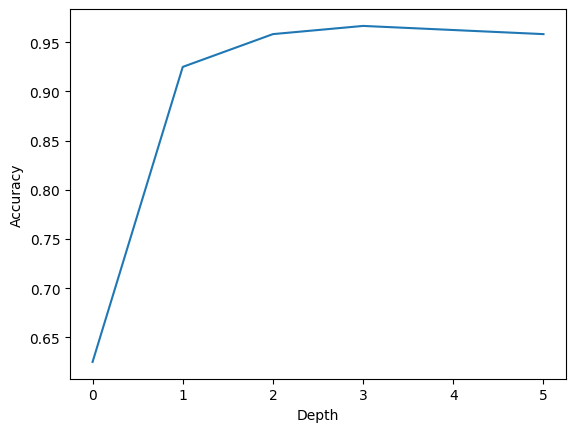
\includegraphics{Assignment6_Final version_files/figure-pdf/cell-31-output-1.png}

\begin{Shaded}
\begin{Highlighting}[]
\NormalTok{cs\_dt\_best }\OperatorTok{=}\NormalTok{ DecisionTreeClassifier(}
\NormalTok{    max\_depth }\OperatorTok{=} \DecValTok{3}\NormalTok{, }
\NormalTok{    random\_state}\OperatorTok{=}\DecValTok{1}
\NormalTok{    ) }
\NormalTok{cs\_dt\_best.fit(X\_train, y\_train)}
\end{Highlighting}
\end{Shaded}

\begin{verbatim}
DecisionTreeClassifier(max_depth=3, random_state=1)
\end{verbatim}

\begin{Shaded}
\begin{Highlighting}[]
\NormalTok{X\_train, X\_test, y\_train, y\_test }\OperatorTok{=}\NormalTok{ train\_test\_split(}
\NormalTok{    X, y, test\_size}\OperatorTok{=}\FloatTok{0.3}\NormalTok{, random\_state}\OperatorTok{=}\DecValTok{1}\NormalTok{, stratify}\OperatorTok{=}\NormalTok{y)}
\NormalTok{plot\_tree(}
\NormalTok{    cs\_dt\_best, }
\NormalTok{    max\_depth}\OperatorTok{=} \DecValTok{3}\NormalTok{, }
\NormalTok{    feature\_names }\OperatorTok{=}\NormalTok{ X\_train.columns.tolist(), }
\NormalTok{    filled}\OperatorTok{=}\VariableTok{True}\NormalTok{,}
\NormalTok{    class\_names}\OperatorTok{=}\NormalTok{[}\StringTok{\textquotesingle{}notckd\textquotesingle{}}\NormalTok{, }\StringTok{\textquotesingle{}ckd\textquotesingle{}}\NormalTok{]}
\NormalTok{)}

\NormalTok{pred\_BDT }\OperatorTok{=}\NormalTok{ cs\_dt.predict(X\_test)}

\BuiltInTok{print}\NormalTok{(classification\_report(y\_test, pred\_BDT))}
\NormalTok{cm\_BDT }\OperatorTok{=}\NormalTok{ pd.DataFrame(confusion\_matrix(y\_test, pred\_BDT), index}\OperatorTok{=}\NormalTok{[}\StringTok{\textquotesingle{}No\textquotesingle{}}\NormalTok{, }\StringTok{\textquotesingle{}Yes\textquotesingle{}}\NormalTok{], columns}\OperatorTok{=}\NormalTok{[}\StringTok{\textquotesingle{}No\textquotesingle{}}\NormalTok{, }\StringTok{\textquotesingle{}Yes\textquotesingle{}}\NormalTok{])}
\NormalTok{cm\_BDT.index.name }\OperatorTok{=} \StringTok{\textquotesingle{}True\textquotesingle{}}
\NormalTok{cm\_BDT.columns.name }\OperatorTok{=} \StringTok{\textquotesingle{}Predicted\textquotesingle{}}

\BuiltInTok{print}\NormalTok{(cm\_BDT)}
\NormalTok{cs\_dt.score(X\_test, y\_test)}
\BuiltInTok{print}\NormalTok{(}\StringTok{"Accuracy:"}\NormalTok{, accuracy\_score(y\_test, pred\_BDT))}
\end{Highlighting}
\end{Shaded}

\begin{verbatim}
              precision    recall  f1-score   support

         ckd       0.96      0.97      0.97        75
      notckd       0.95      0.93      0.94        45

    accuracy                           0.96       120
   macro avg       0.96      0.95      0.96       120
weighted avg       0.96      0.96      0.96       120

Predicted  No  Yes
True              
No         73    2
Yes         3   42
Accuracy: 0.9583333333333334
\end{verbatim}

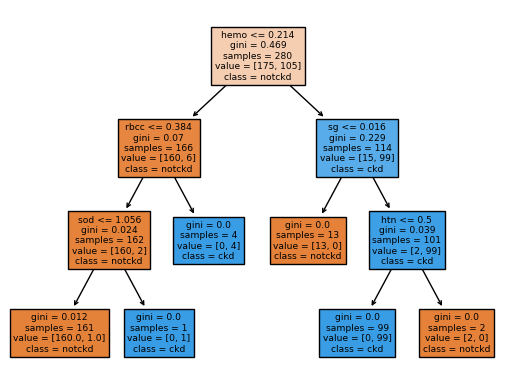
\includegraphics{Assignment6_Final version_files/figure-pdf/cell-33-output-2.png}

\begin{Shaded}
\begin{Highlighting}[]
\NormalTok{fea\_imp }\OperatorTok{=}\NormalTok{ cs\_dt\_best.feature\_importances\_}
\NormalTok{sorted\_indices }\OperatorTok{=}\NormalTok{ fea\_imp.argsort()[::}\OperatorTok{{-}}\DecValTok{1}\NormalTok{]}
\NormalTok{sorted\_feature\_names }\OperatorTok{=}\NormalTok{ X\_train.columns[sorted\_indices]}
\NormalTok{sorted\_importances }\OperatorTok{=}\NormalTok{ fea\_imp[sorted\_indices]}
\NormalTok{sns.barplot(x }\OperatorTok{=}\NormalTok{ sorted\_importances, y }\OperatorTok{=}\NormalTok{ sorted\_feature\_names)}
\NormalTok{plt.ylabel(}\StringTok{"variables"}\NormalTok{)}

\NormalTok{plt.show()}
\end{Highlighting}
\end{Shaded}

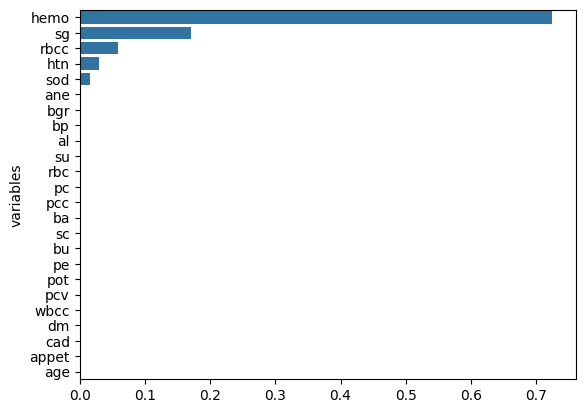
\includegraphics{Assignment6_Final version_files/figure-pdf/cell-34-output-1.png}

From above plot, we can observe variable ``hemo'' has a significant
influce on the model, next is ``sg'' and ``rbcc''. ``htn'' and ``sod''
also have some influence. Rest of the variables do not have a crucial
impact on the model. After pruning the tree, we can see the acuracy did
not increase. That is mostly because the previous one has a really large
depth, but even with a max depth of 3, the model can achieve the same
accuracy. Simplifing the model can also be seen as an improvement.

\begin{Shaded}
\begin{Highlighting}[]

\NormalTok{X\_train, X\_test, y\_train, y\_test }\OperatorTok{=}\NormalTok{ train\_test\_split(}
\NormalTok{    X, y, test\_size}\OperatorTok{=}\FloatTok{0.3}\NormalTok{, random\_state}\OperatorTok{=}\DecValTok{1}\NormalTok{, stratify}\OperatorTok{=}\NormalTok{y)}
\NormalTok{clf }\OperatorTok{=}\NormalTok{ DecisionTreeClassifier(max\_depth }\OperatorTok{=}\DecValTok{30}\NormalTok{, }
\NormalTok{    random\_state}\OperatorTok{=}\DecValTok{1}\NormalTok{,criterion}\OperatorTok{=}\StringTok{\textquotesingle{}entropy\textquotesingle{}}\NormalTok{)  }
\NormalTok{clf.fit(X\_train, y\_train)}


\NormalTok{pred\_clf }\OperatorTok{=}\NormalTok{ clf.predict(X\_test)}


\BuiltInTok{print}\NormalTok{(}\StringTok{"Accuracy:"}\NormalTok{, accuracy\_score(y\_test, pred\_clf))}
\BuiltInTok{print}\NormalTok{(classification\_report(y\_test, pred\_clf))}


\NormalTok{plt.figure(figsize}\OperatorTok{=}\NormalTok{(}\DecValTok{10}\NormalTok{,}\DecValTok{6}\NormalTok{))}
\NormalTok{plot\_tree(clf, filled}\OperatorTok{=}\VariableTok{True}\NormalTok{,feature\_names }\OperatorTok{=}\NormalTok{ X\_train.columns.tolist(),class\_names}\OperatorTok{=}\NormalTok{[}\StringTok{\textquotesingle{}notckd\textquotesingle{}}\NormalTok{, }\StringTok{\textquotesingle{}ckd\textquotesingle{}}\NormalTok{])}
\NormalTok{plt.show()}
\end{Highlighting}
\end{Shaded}

\begin{verbatim}
Accuracy: 0.9666666666666667
              precision    recall  f1-score   support

         ckd       0.96      0.99      0.97        75
      notckd       0.98      0.93      0.95        45

    accuracy                           0.97       120
   macro avg       0.97      0.96      0.96       120
weighted avg       0.97      0.97      0.97       120
\end{verbatim}

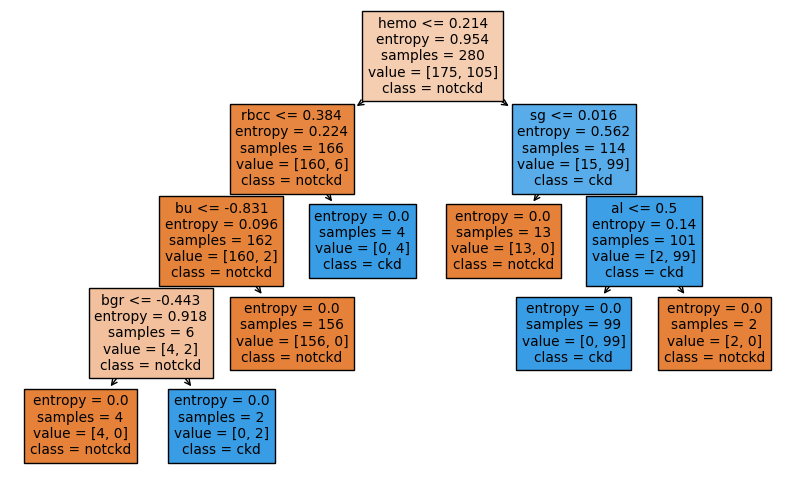
\includegraphics{Assignment6_Final version_files/figure-pdf/cell-35-output-2.png}

The next method we used for improving the model is to change the
crierion. The improvement of accuracy scores indicates a better result,
which implies we have a better model.

\begin{Shaded}
\begin{Highlighting}[]
\NormalTok{cm\_clf }\OperatorTok{=}\NormalTok{ pd.DataFrame(confusion\_matrix(y\_test, pred\_clf), index}\OperatorTok{=}\NormalTok{[}\StringTok{\textquotesingle{}No\textquotesingle{}}\NormalTok{, }\StringTok{\textquotesingle{}Yes\textquotesingle{}}\NormalTok{], columns}\OperatorTok{=}\NormalTok{[}\StringTok{\textquotesingle{}No\textquotesingle{}}\NormalTok{, }\StringTok{\textquotesingle{}Yes\textquotesingle{}}\NormalTok{])}
\NormalTok{cm\_clf.index.name }\OperatorTok{=} \StringTok{\textquotesingle{}True\textquotesingle{}}
\NormalTok{cm\_clf.columns.name }\OperatorTok{=} \StringTok{\textquotesingle{}Predicted\textquotesingle{}}
\NormalTok{cm\_clf}
\end{Highlighting}
\end{Shaded}

\begin{longtable}[]{@{}lll@{}}
\toprule\noalign{}
Predicted & No & Yes \\
True & & \\
\midrule\noalign{}
\endhead
\bottomrule\noalign{}
\endlastfoot
No & 74 & 1 \\
Yes & 3 & 42 \\
\end{longtable}

Like we mentioned above, we will use mean for missing numerical datas,
and most frequent more categorical data.

\begin{Shaded}
\begin{Highlighting}[]
\NormalTok{float\_col }\OperatorTok{=}\NormalTok{ X[numerical\_cols].columns.tolist()}
\NormalTok{num\_imputer }\OperatorTok{=}\NormalTok{ SimpleImputer(missing\_values}\OperatorTok{=}\NormalTok{np.nan,strategy}\OperatorTok{=}\StringTok{\textquotesingle{}mean\textquotesingle{}}\NormalTok{)}
\NormalTok{X.loc[:, float\_col] }\OperatorTok{=}\NormalTok{ num\_imputer.fit\_transform(X.loc[:, float\_col])}

\CommentTok{\# For categorical features}
\NormalTok{obj\_col }\OperatorTok{=}\NormalTok{ X[categorcal\_cols].columns.tolist()}
\NormalTok{cat\_imputer }\OperatorTok{=}\NormalTok{ SimpleImputer(strategy}\OperatorTok{=}\StringTok{\textquotesingle{}most\_frequent\textquotesingle{}}\NormalTok{,missing\_values}\OperatorTok{=}\NormalTok{np.nan)}
\NormalTok{X.loc[:, obj\_col] }\OperatorTok{=}\NormalTok{ cat\_imputer.fit\_transform(X.loc[:, obj\_col])}
\end{Highlighting}
\end{Shaded}

\begin{Shaded}
\begin{Highlighting}[]
\NormalTok{X.isna().}\BuiltInTok{sum}\NormalTok{()}
\end{Highlighting}
\end{Shaded}

\begin{verbatim}
age      0
bp       0
sg       0
al       0
su       0
rbc      0
pc       0
pcc      0
ba       0
bgr      0
bu       0
sc       0
sod      0
pot      0
hemo     0
pcv      0
wbcc     0
rbcc     0
htn      0
dm       0
cad      0
appet    0
pe       0
ane      0
dtype: int64
\end{verbatim}

\begin{Shaded}
\begin{Highlighting}[]
\NormalTok{X\_train, X\_test, y\_train, y\_test }\OperatorTok{=}\NormalTok{ train\_test\_split(}
\NormalTok{    X, y, test\_size}\OperatorTok{=}\FloatTok{0.3}\NormalTok{, random\_state}\OperatorTok{=}\DecValTok{1}\NormalTok{, stratify}\OperatorTok{=}\NormalTok{y)}
\end{Highlighting}
\end{Shaded}

\begin{Shaded}
\begin{Highlighting}[]
\CommentTok{\# Initialize and train SVM model}
\NormalTok{svm }\OperatorTok{=}\NormalTok{ SVC(kernel}\OperatorTok{=}\StringTok{\textquotesingle{}linear\textquotesingle{}}\NormalTok{)}
\NormalTok{y\_train }\OperatorTok{=}\NormalTok{ np.ravel(y\_train)}
\NormalTok{svm.fit(X\_train, y\_train)}

\end{Highlighting}
\end{Shaded}

\begin{verbatim}
SVC(kernel='linear')
\end{verbatim}

\section{12}\label{section-6}

\begin{Shaded}
\begin{Highlighting}[]
\NormalTok{cm }\OperatorTok{=}\NormalTok{ confusion\_matrix(y\_test, pred\_clf)}
\BuiltInTok{print}\NormalTok{(}\StringTok{\textquotesingle{}Confusion Matrix from Decicion Tree: }\CharTok{\textbackslash{}n}\StringTok{\textquotesingle{}}\NormalTok{, cm)}
\NormalTok{accuracyDT }\OperatorTok{=}\NormalTok{ accuracy\_score(y\_test, pred\_clf)}
\BuiltInTok{print}\NormalTok{(}\StringTok{"Accuracy from SVM:"}\NormalTok{, accuracyDT)}
\end{Highlighting}
\end{Shaded}

\begin{verbatim}
Confusion Matrix from Decicion Tree: 
 [[74  1]
 [ 3 42]]
Accuracy from SVM: 0.9666666666666667
\end{verbatim}

\begin{Shaded}
\begin{Highlighting}[]
\NormalTok{y\_pred\_SVM }\OperatorTok{=}\NormalTok{ svm.predict(X\_test)}
\NormalTok{accuracy }\OperatorTok{=}\NormalTok{ accuracy\_score(y\_test, y\_pred\_SVM)}
\NormalTok{cm\_SVM }\OperatorTok{=}\NormalTok{ confusion\_matrix(y\_test, y\_pred\_SVM)}
\BuiltInTok{print}\NormalTok{(}\StringTok{\textquotesingle{}Confusion Matrix from Decicion Tree: }\CharTok{\textbackslash{}n}\StringTok{\textquotesingle{}}\NormalTok{, cm\_SVM)}
\BuiltInTok{print}\NormalTok{(}\StringTok{"Accuracy from SVM:"}\NormalTok{, accuracy)}
\end{Highlighting}
\end{Shaded}

\begin{verbatim}
Confusion Matrix from Decicion Tree: 
 [[75  0]
 [ 2 43]]
Accuracy from SVM: 0.9833333333333333
\end{verbatim}

By comparing the confusion matrix and accuarcy score, we can conclude
that linear SVC is a more suitable model for this dataset.

\section{13}\label{section-7}

\begin{Shaded}
\begin{Highlighting}[]
\NormalTok{fea\_imp }\OperatorTok{=}\NormalTok{ clf.feature\_importances\_}
\NormalTok{sorted\_indices }\OperatorTok{=}\NormalTok{ fea\_imp.argsort()[::}\OperatorTok{{-}}\DecValTok{1}\NormalTok{]}
\NormalTok{sorted\_feature\_names }\OperatorTok{=}\NormalTok{ X\_train.columns[sorted\_indices]}
\NormalTok{sorted\_importances }\OperatorTok{=}\NormalTok{ fea\_imp[sorted\_indices]}
\NormalTok{sns.barplot(x }\OperatorTok{=}\NormalTok{ sorted\_importances, y }\OperatorTok{=}\NormalTok{ sorted\_feature\_names)}
\NormalTok{plt.ylabel(}\StringTok{"variables"}\NormalTok{)}

\NormalTok{plt.show()}
\end{Highlighting}
\end{Shaded}

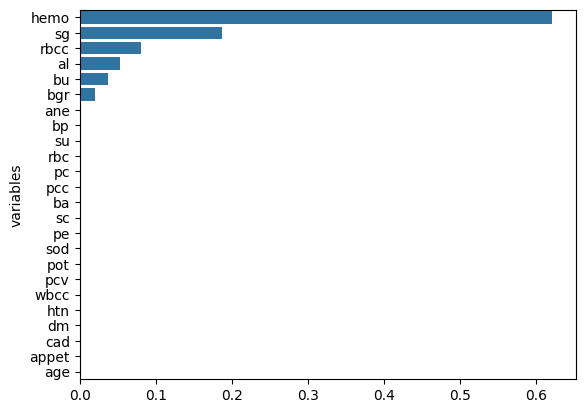
\includegraphics{Assignment6_Final version_files/figure-pdf/cell-43-output-1.png}

\section{14}\label{section-8}

\begin{Shaded}
\begin{Highlighting}[]
\ImportTok{from}\NormalTok{ sklearn.preprocessing }\ImportTok{import}\NormalTok{ PolynomialFeatures}
\ImportTok{from}\NormalTok{ sklearn.metrics }\ImportTok{import}\NormalTok{ accuracy\_score}


\NormalTok{X\_train, X\_test, y\_train, y\_test }\OperatorTok{=}\NormalTok{ train\_test\_split(}
\NormalTok{    new\_X, new\_y, test\_size}\OperatorTok{=}\FloatTok{0.3}\NormalTok{, random\_state}\OperatorTok{=}\DecValTok{1}\NormalTok{, stratify}\OperatorTok{=}\NormalTok{new\_y)}


\NormalTok{poly}\OperatorTok{=}\NormalTok{PolynomialFeatures(degree}\OperatorTok{=}\DecValTok{2}\NormalTok{, interaction\_only}\OperatorTok{=}\VariableTok{True}\NormalTok{)}
\NormalTok{X\_train\_poly }\OperatorTok{=}\NormalTok{ poly.fit\_transform(X\_train)}
\NormalTok{X\_test\_poly }\OperatorTok{=}\NormalTok{ poly.transform(X\_test)}


\NormalTok{DTC }\OperatorTok{=}\NormalTok{ DecisionTreeClassifier(max\_depth }\OperatorTok{=}\DecValTok{3}\NormalTok{, }
\NormalTok{    random\_state}\OperatorTok{=}\DecValTok{1}\NormalTok{,criterion}\OperatorTok{=}\StringTok{\textquotesingle{}entropy\textquotesingle{}}\NormalTok{) }


\NormalTok{DTC.fit(X\_train\_poly, y\_train)}


\NormalTok{y\_pred\_poly }\OperatorTok{=}\NormalTok{ DTC.predict(X\_test\_poly)}
\NormalTok{accuracy\_poly }\OperatorTok{=}\NormalTok{ accuracy\_score(y\_test, y\_pred\_poly)}
\BuiltInTok{print}\NormalTok{(}\StringTok{"New Model Accuracy:"}\NormalTok{, accuracy\_poly)}
\end{Highlighting}
\end{Shaded}

\begin{verbatim}
New Model Accuracy: 0.9791666666666666
\end{verbatim}

The improved model does not bring us a better result. It is may because
polynomial features introduce interaction terms between features, and
sometimes there may be cases these interactions may not be relevant or
may even introduce noise, leading to overfitting. It also increase the
dimension of the model where a overly complicated model may not be as
accurate as a simplier one.

\section{15 Distribution}\label{distribution}

Tianmu Li (400371751): Question 2, 3, 4, 5, 6, 11

Chengdai Xu (400397089): Question 5, 7, 8, 9, 10, 11,14

Jiajun Zhang (400359213) : Question 1, 3, 7, 11, 12, 13

We have done a lot of work together by sharing the jupyter file itself
instead of using github, but all of the questions are done under
continuously disscussion and communication in the group. The
contribution of each team members are equal and fair.



\end{document}
